%#!platex ./report.tex
   
\section{Ka$B%A%c%M%k(B, CaT$B%A%c%M%k$rMQ$$$?>l9g$N7k2L(B}
$B?^(B\ref{k_ca_result1}, $B?^(B\ref{k_ca_result2}, $B?^(B\ref{k_ca_result3}$B$K(BKa$B%A%c%M%k(B, CaT$B%A%c%M%k$rN>J}F3F~$7$?>l9g$N(B
$B7k2L$r<($9(B. $B?^Cf$NK^Nc$d8!Dj<jK!$H$=$N7k2L$N<($7J}$O?^(B\ref{Ka_Result1}$B$HF1MM$G$"$k(B.
   
     \begin{figure}[H]
       \begin{subfigure}{0.5\columnwidth}
         \centering
         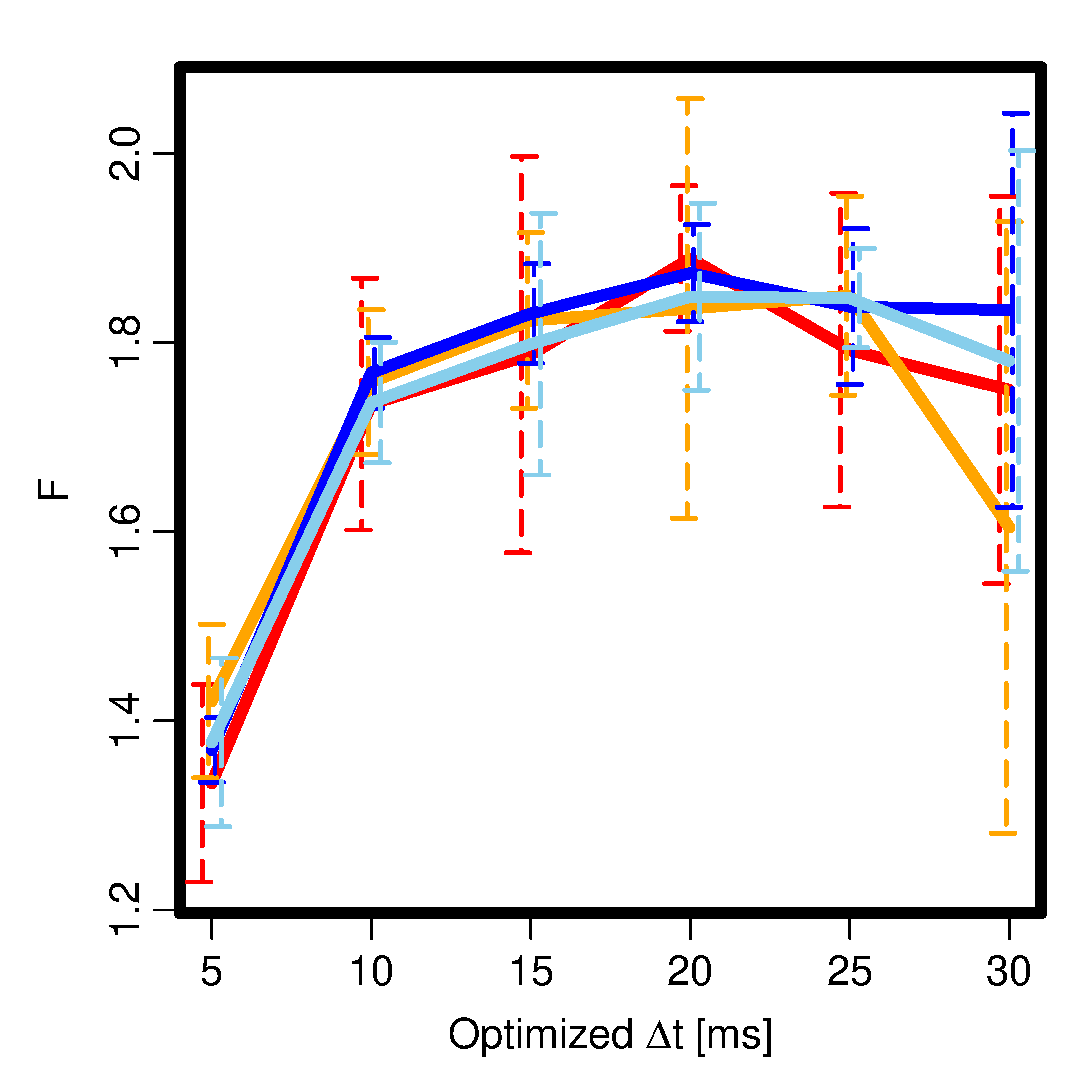
\includegraphics[width=0.8\columnwidth]{./Images_Result/k_ca_test_F.eps}
         \caption{$F$}
         \label{k_ca_F}
       \end{subfigure}
       \begin{subfigure}{0.5\columnwidth}
         \centering
         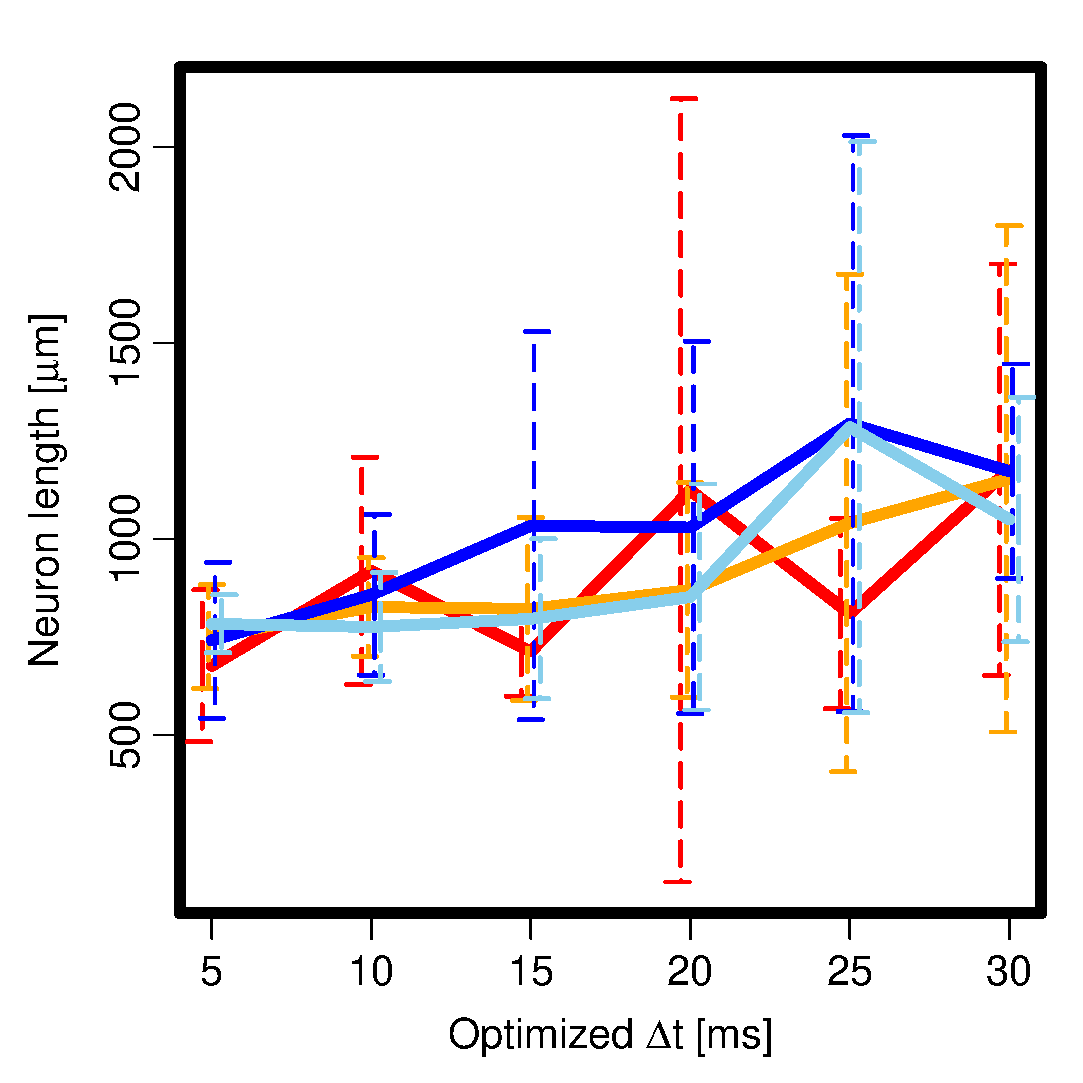
\includegraphics[width=0.8\columnwidth]{./Images_Result/k_ca_test_TREE_length.eps} 
         \caption{$BD9$5(B}
         \label{k_ca_TREE_length}
       \end{subfigure}

       \begin{subfigure}{0.5\columnwidth}
         \centering
         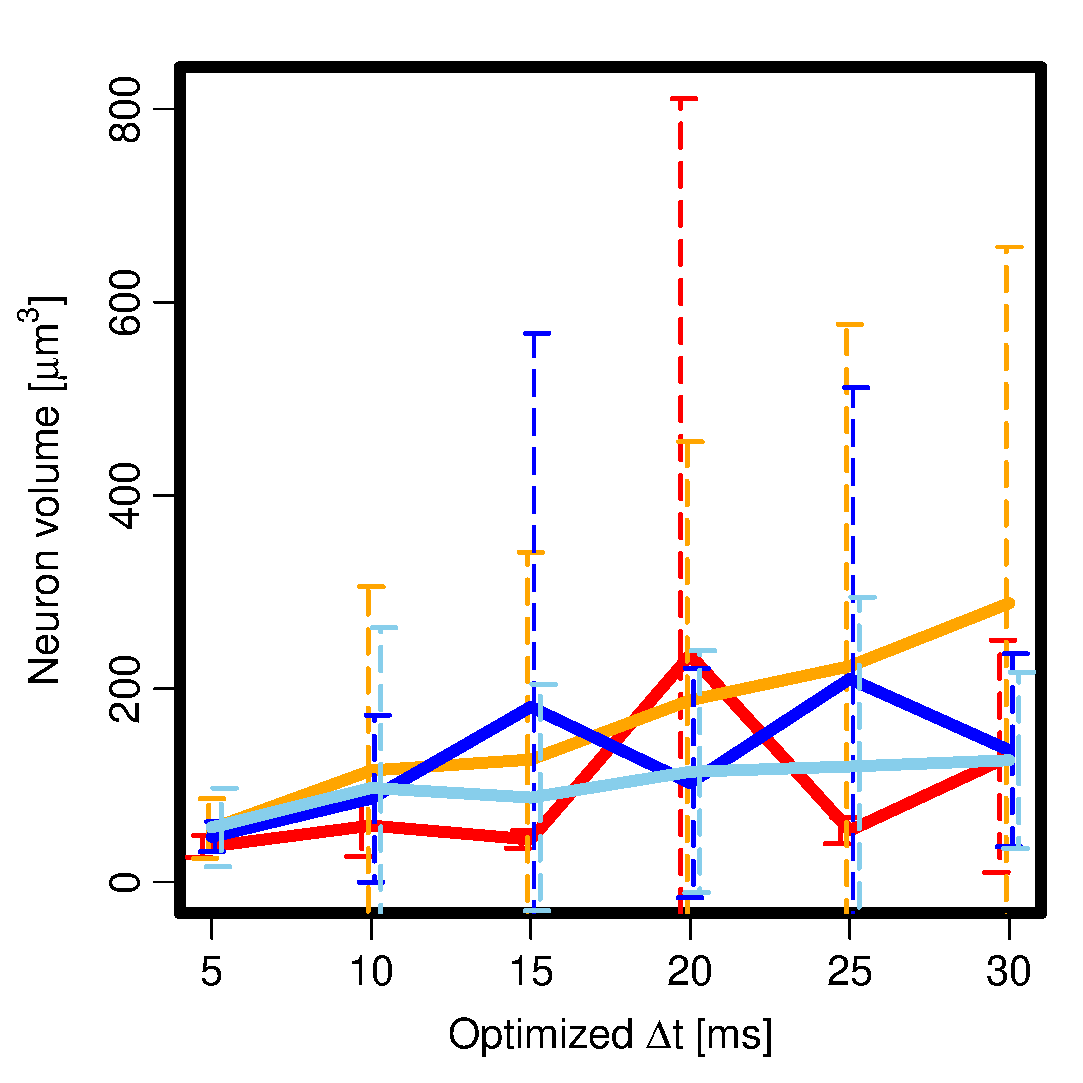
\includegraphics[width=0.8\columnwidth]{./Images_Result/k_ca_test_TREE_volume.eps}
         \caption{$BBN@Q(B}
         \label{k_ca_TREE_volume}
       \end{subfigure}
       \begin{subfigure}{0.5\columnwidth}
         \centering
         \hspace*{-1cm}
         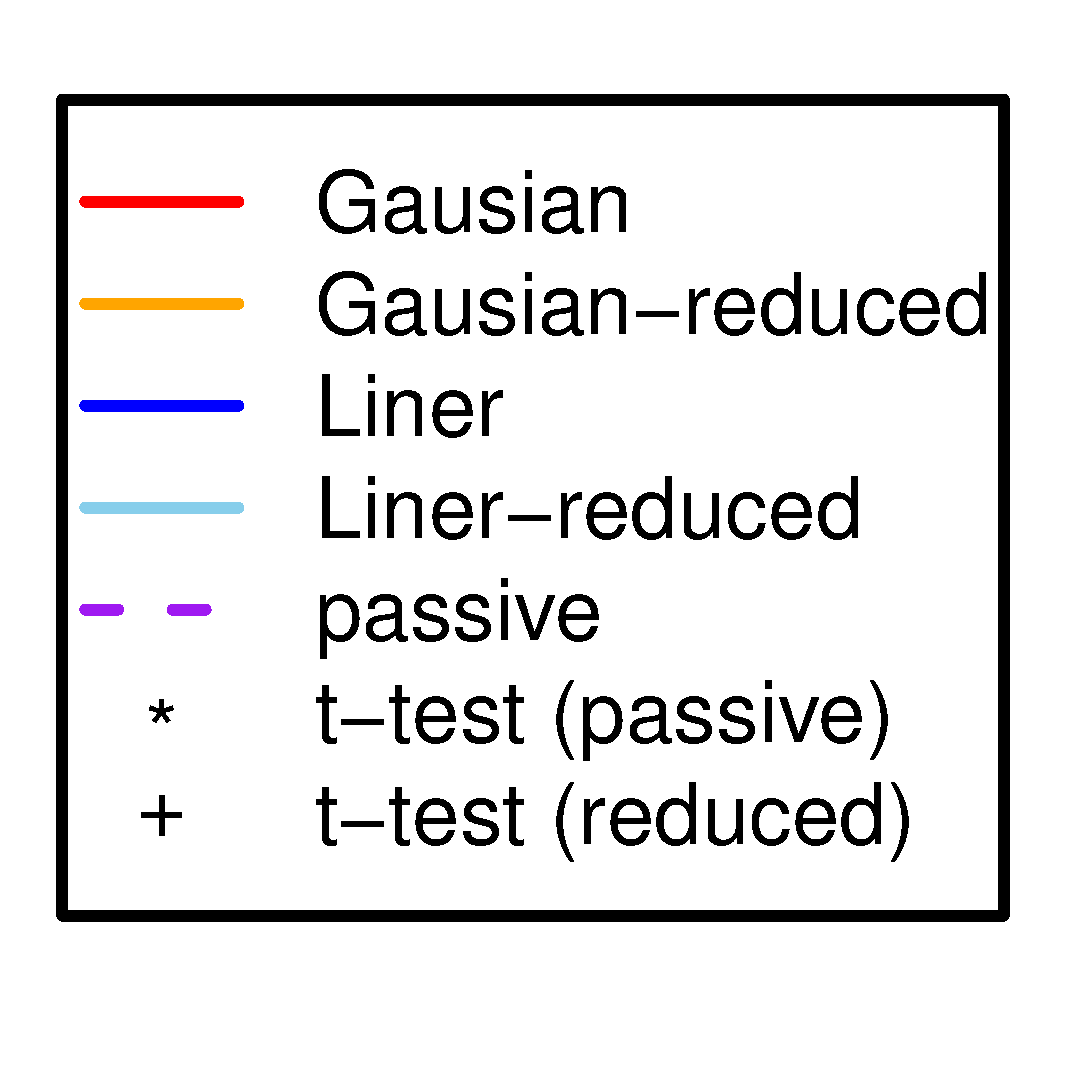
\includegraphics[width=0.5\columnwidth]{./Images_Result/ca_test_legend.eps}
         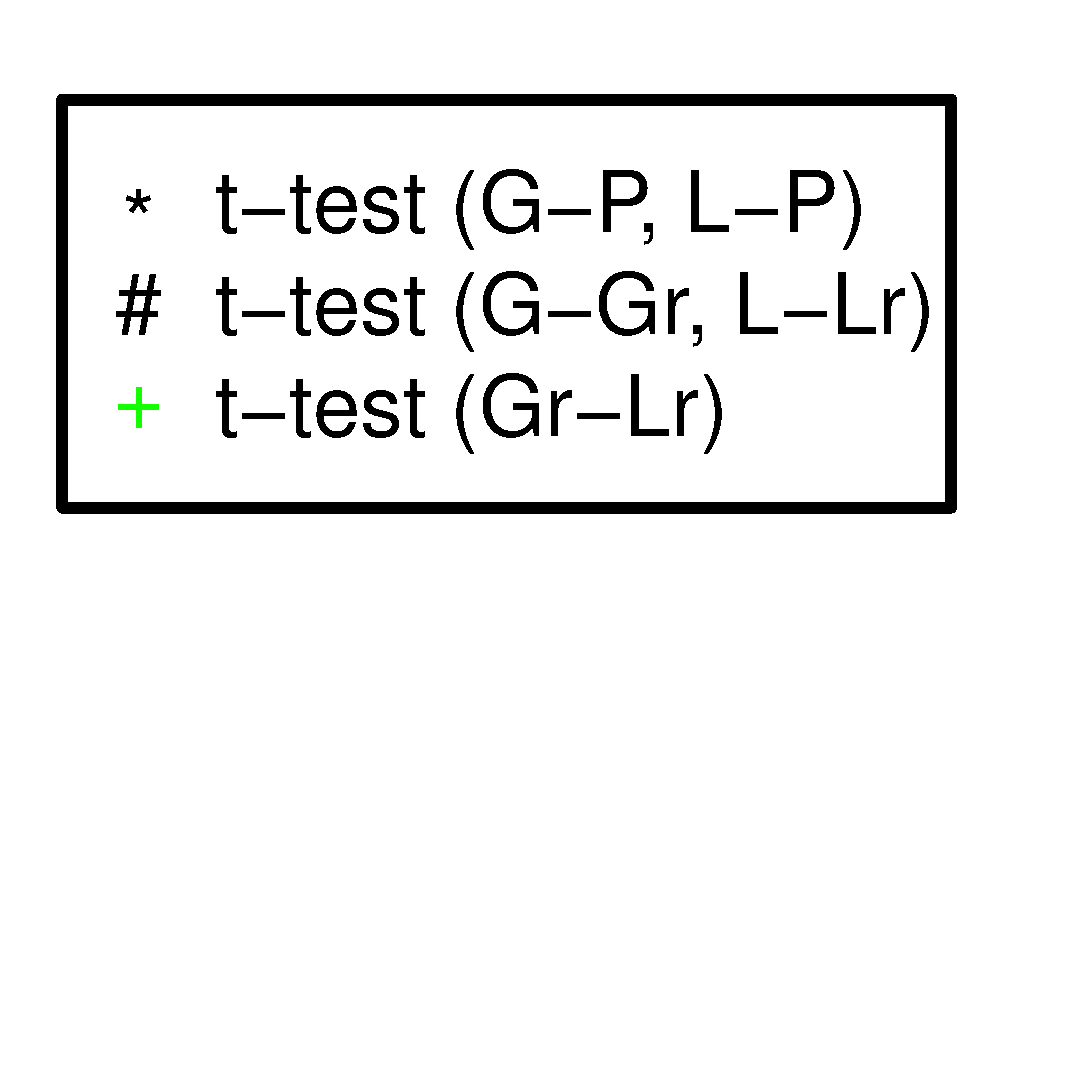
\includegraphics[width=0.5\columnwidth]{./Images_Result/test_legend.eps} 
       \end{subfigure}
              
       \caption{Ka$B%A%c%M%k(B, CaT$B%A%c%M%k$rF3F~$7$?:]$N7k2L(B1} %$B%Z!<%8%l%$%"%&%H$,7hDj$7$F$+$iHyD4@0$9$k(B
       \label{k_ca_result1}
     \end{figure}
     
     $B?^(B\ref{k_ca_F}$B$r8+$k$H(B${\Delta}t = 5$[ms]$B0J30$N>l9g(B, $B$I$N%3%s%@%/%?%s%9J,I[%Q%?!<%s$G$b(B
     $F$$B$NCM$O(B${\Delta}t$$B$K$h$i$:(B1.7$B$+$i(B1.8$B$[$I$K$J$C$?(B. \\

     \begin{figure}[H]
       \begin{subfigure}{0.5\columnwidth}
         \centering
         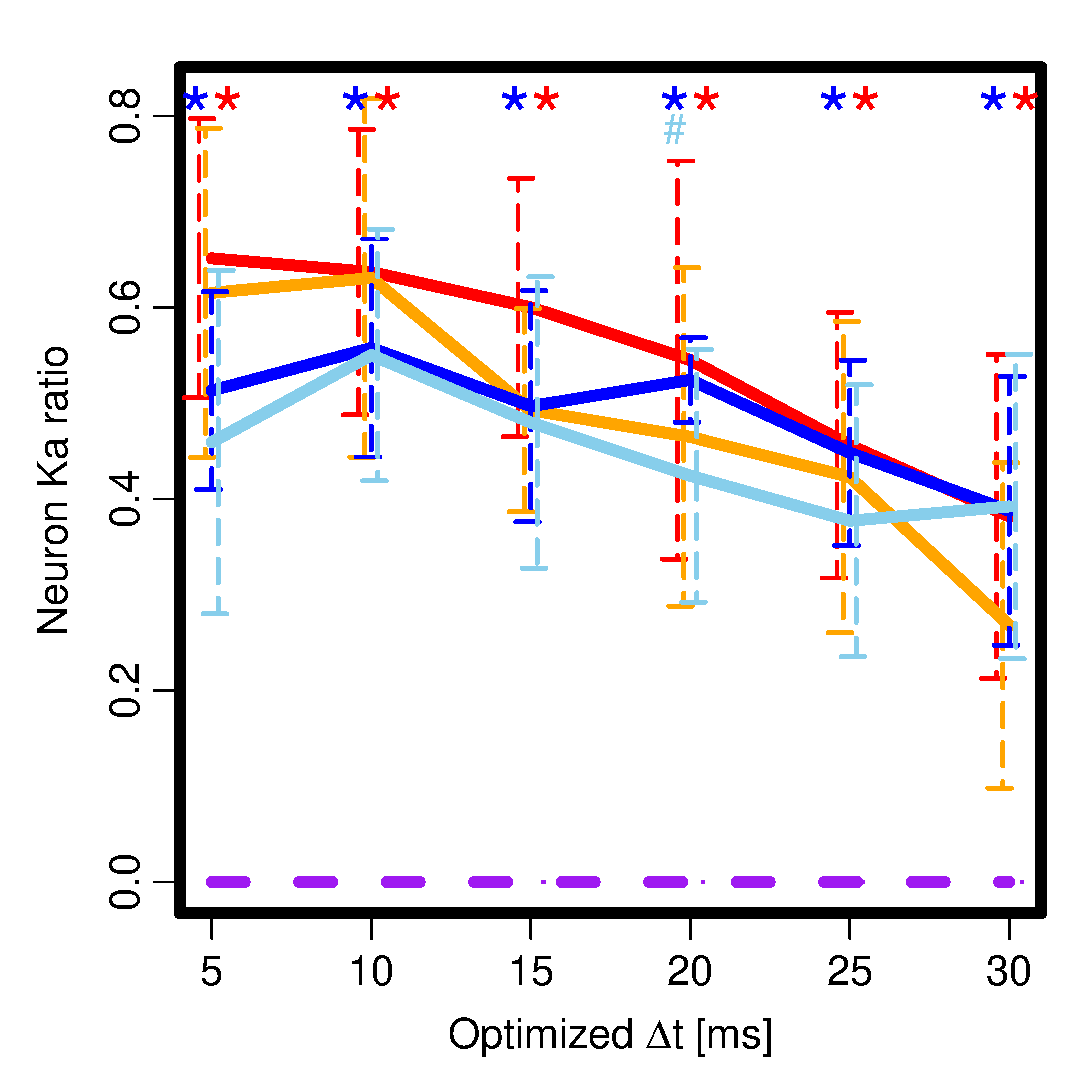
\includegraphics[width=0.8\columnwidth]{./Images_Result/k_ca_test_TREE_K_ratio.eps}
         \caption{Ka$B%3%s%@%/%?%s%94^M-N((B}
         \label{ca_TREE_K_ratio}
       \end{subfigure}
       \begin{subfigure}{0.5\columnwidth}
         \centering
         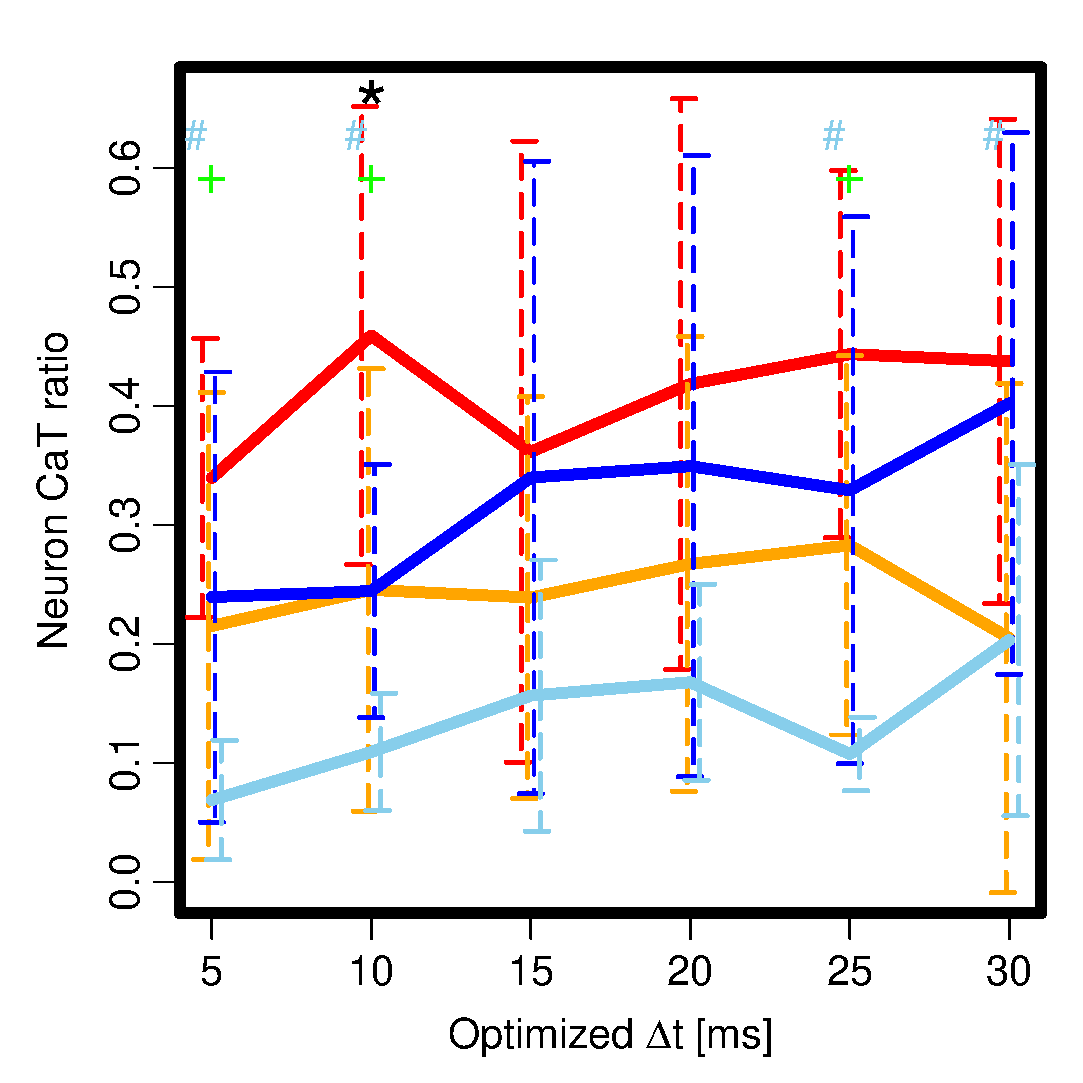
\includegraphics[width=0.8\columnwidth]{./Images_Result/k_ca_test_TREE_Ca_ratio.eps}
         \caption{CaT$B%3%s%@%/%?%s%94^M-N((B}
         \label{ca_TREE_Ca_ratio}
       \end{subfigure}

       \begin{subfigure}{0.5\columnwidth}
         \centering
         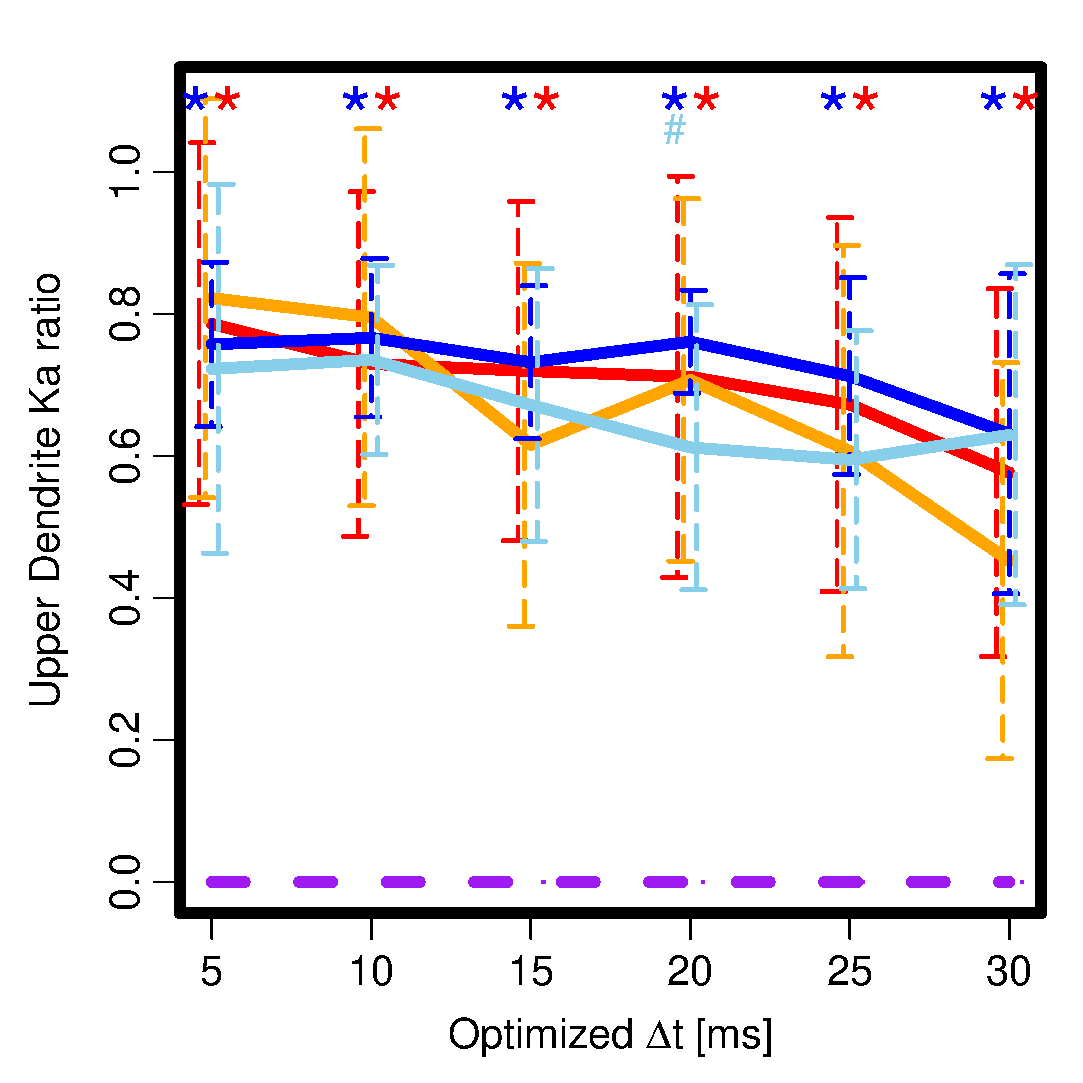
\includegraphics[width=0.8\columnwidth]{./Images_Result/k_ca_test_Upper_K_ratio.eps}
         \caption{Upper Dendrite$B$N(BKa$B%3%s%@%/%?%s%94^M-N((B}
         \label{k_ca_upper_k_ratio}
       \end{subfigure}
       \begin{subfigure}{0.5\columnwidth}
         \centering
         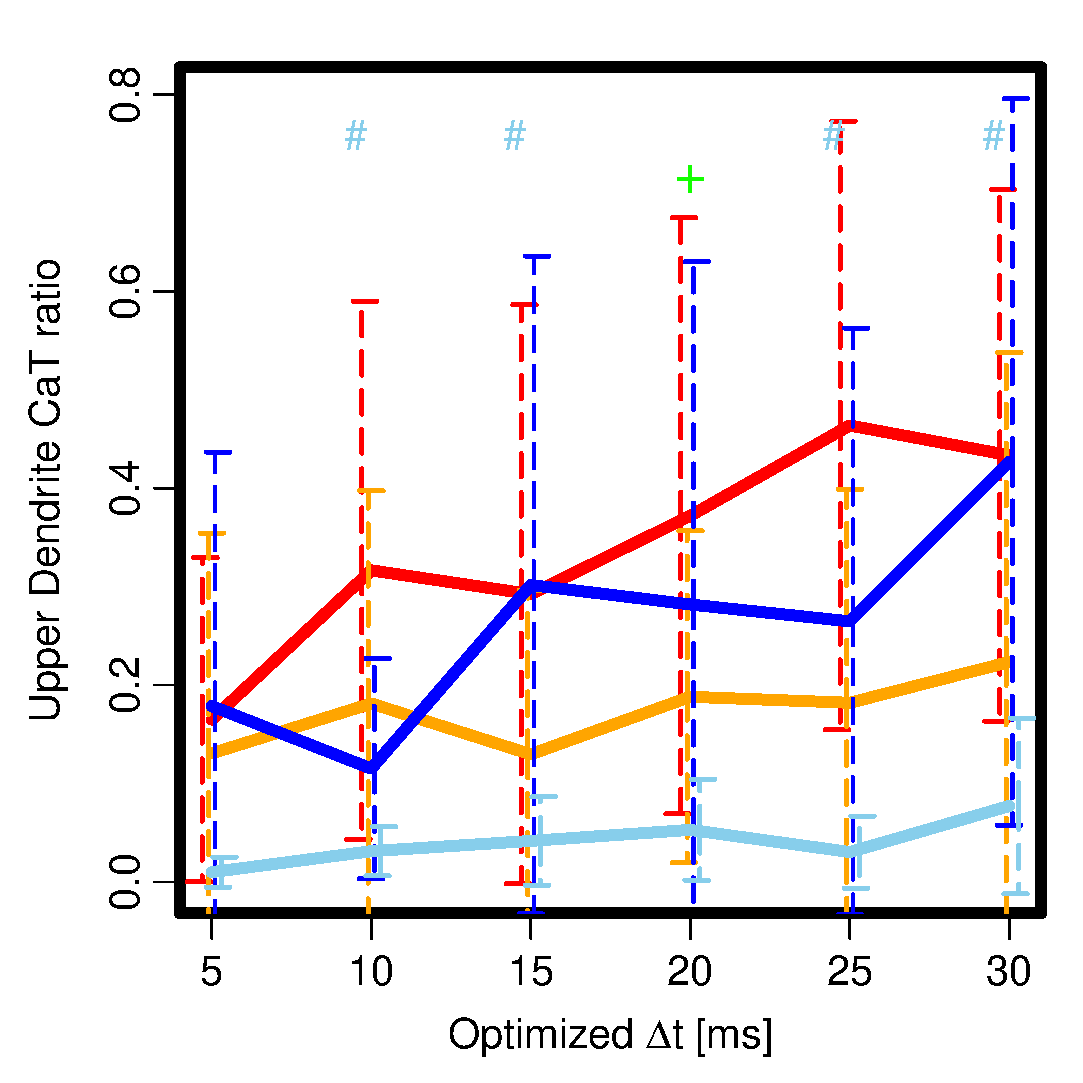
\includegraphics[width=0.8\columnwidth]{./Images_Result/k_ca_test_Upper_Ca_ratio.eps}
         \caption{Upper Dendrite$B$N(BCaT$B%3%s%@%/%?%s%94^M-N((B}
         \label{k_ca_upper_ca_ratio}
       \end{subfigure}

       \begin{subfigure}{0.5\columnwidth}
         \centering
         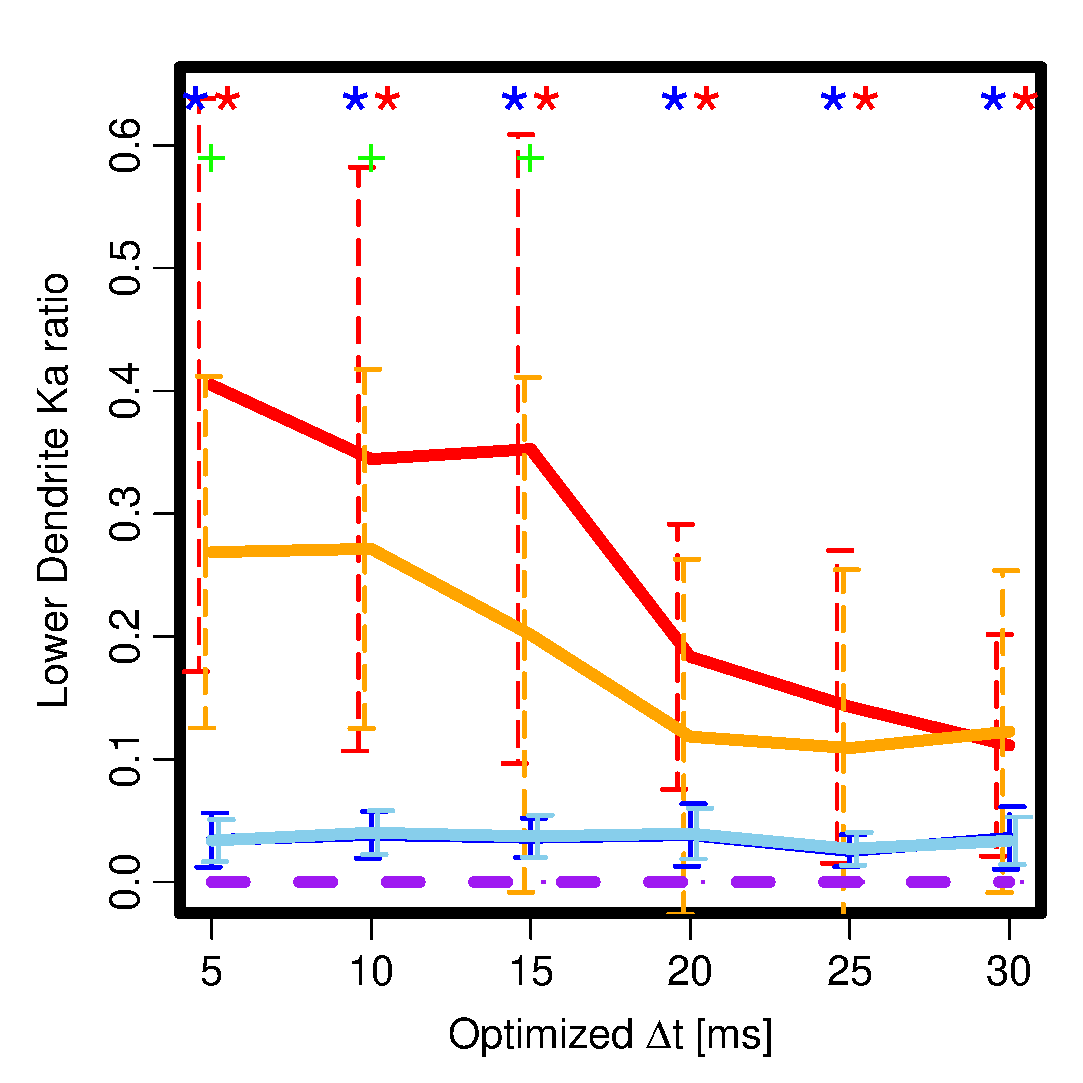
\includegraphics[width=0.8\columnwidth]{./Images_Result/k_ca_test_Lower_K_ratio.eps}
         \caption{Lower Dendrite$B$N(BKa$B%3%s%@%/%?%s%94^M-N((B}
         \label{k_ca_lower_k_ratio}
       \end{subfigure}
       \begin{subfigure}{0.5\columnwidth}
         \centering
         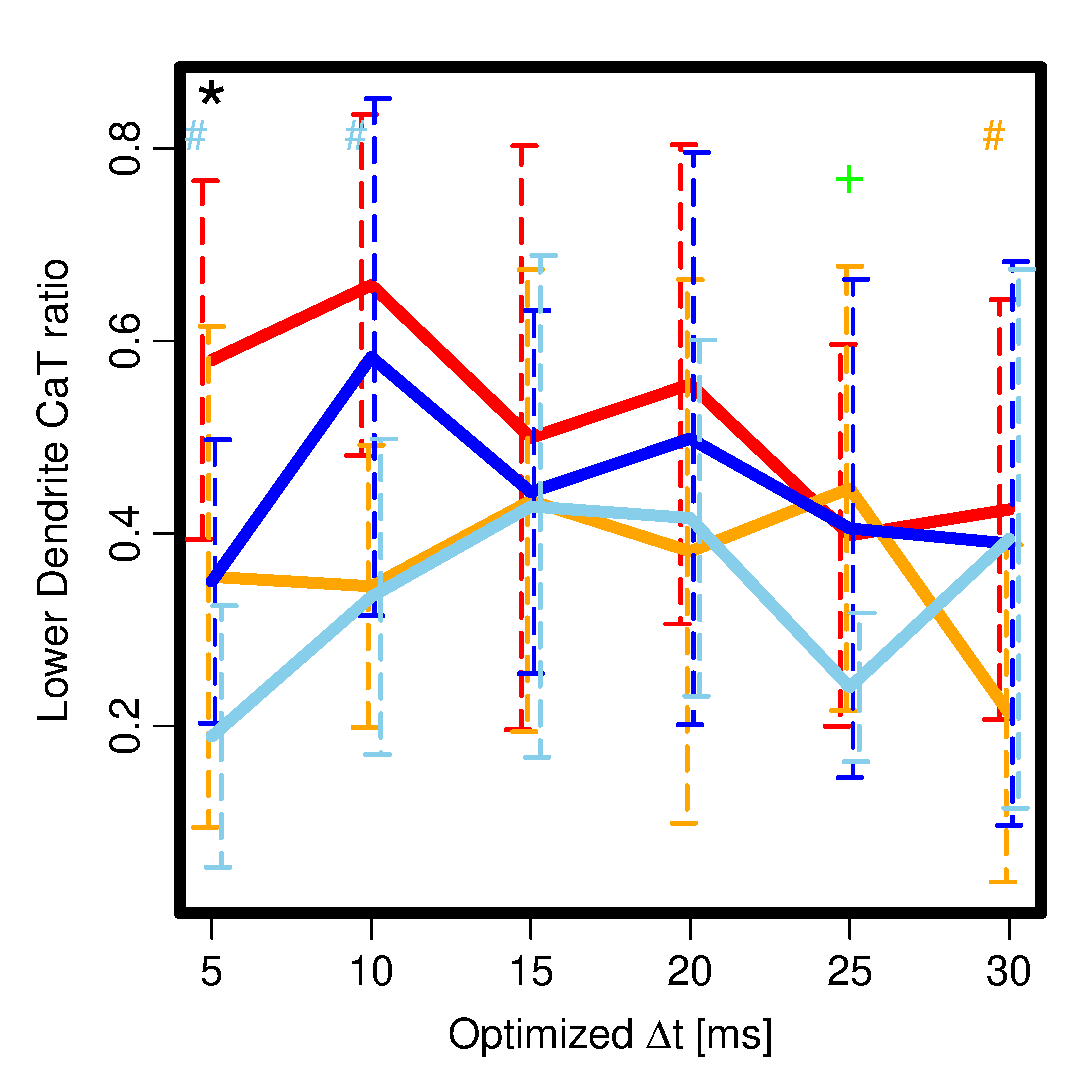
\includegraphics[width=0.8\columnwidth]{./Images_Result/k_ca_test_Lower_Ca_ratio.eps}
         \caption{Lower Dendrite$B$N(BCaT$B%3%s%@%/%?%s%94^M-N((B}
         \label{k_ca_lower_ca_ratio}
       \end{subfigure}

       \caption{Ka$B%A%c%M%k(B, CaT$B%A%c%M%k$rF3F~$7$?:]$N7k2L(B2} %$B%Z!<%8%l%$%"%&%H$,7hDj$7$F$+$iHyD4@0$9$k(B
       \label{k_ca_result2}
     \end{figure}



     \begin{figure}[H]
       \begin{subfigure}{0.5\columnwidth}
         \centering
         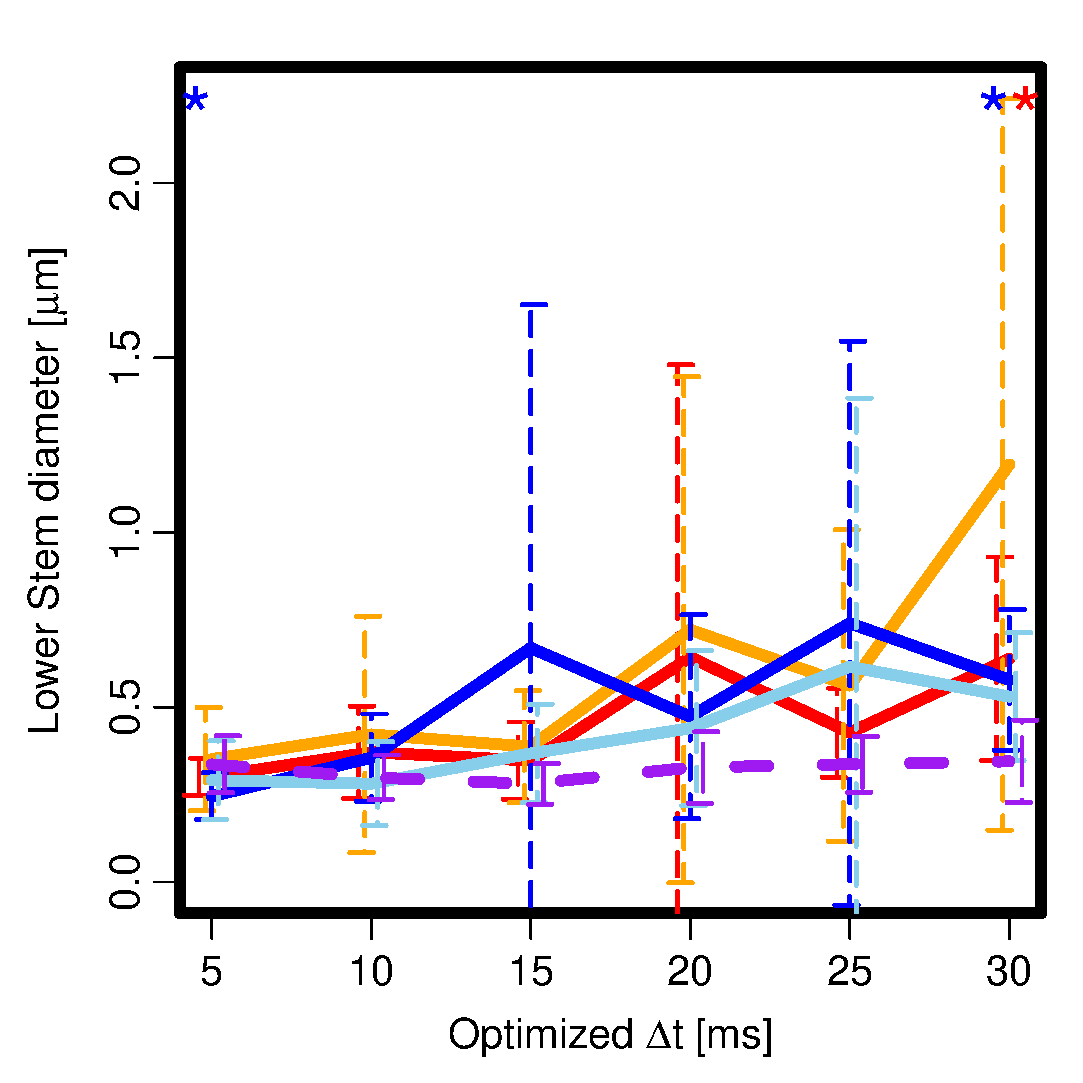
\includegraphics[width=0.8\columnwidth]{./Images_Result/k_ca_test_Lower_Diam.eps}
         \caption{Lower Dend$B$ND>7B(B}
         \label{k_ca_Lower_Diam}
       \end{subfigure}
       \begin{subfigure}{0.5\columnwidth}
         \centering
         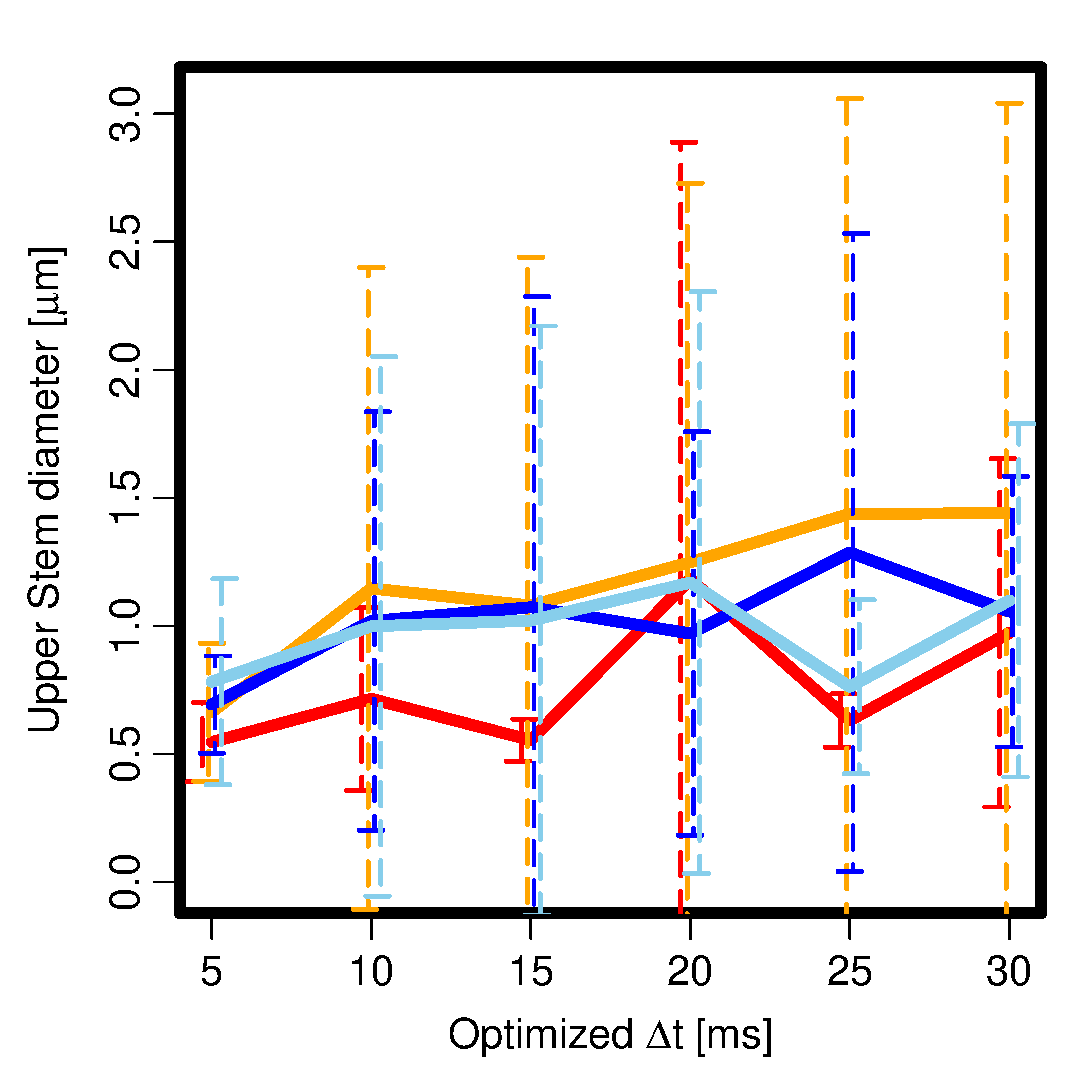
\includegraphics[width=0.8\columnwidth]{./Images_Result/k_ca_test_Upper_Diam.eps}
         \caption{Upper Dend$B$ND>7B(B}
         \label{k_ca_Upper_Diam}
       \end{subfigure}

       \begin{subfigure}{0.5\columnwidth}
         \centering
         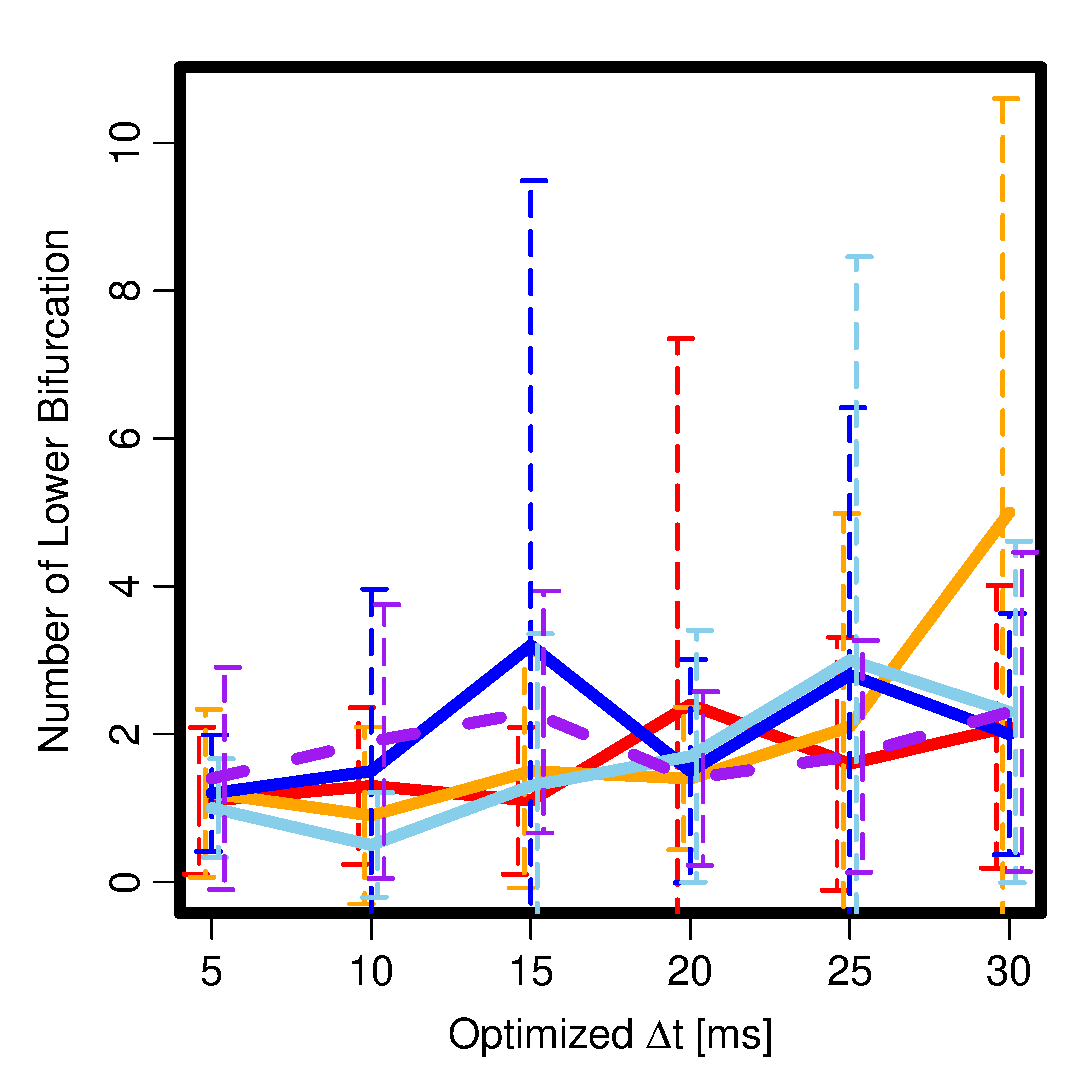
\includegraphics[width=0.8\columnwidth]{./Images_Result/k_ca_test_N_Lower_bif.eps}
         \caption{Lower Dend$B$NJ,4t?t(B}
         \label{k_ca_N_Lower_syn}
       \end{subfigure}
       \begin{subfigure}{0.5\columnwidth}
         \centering
         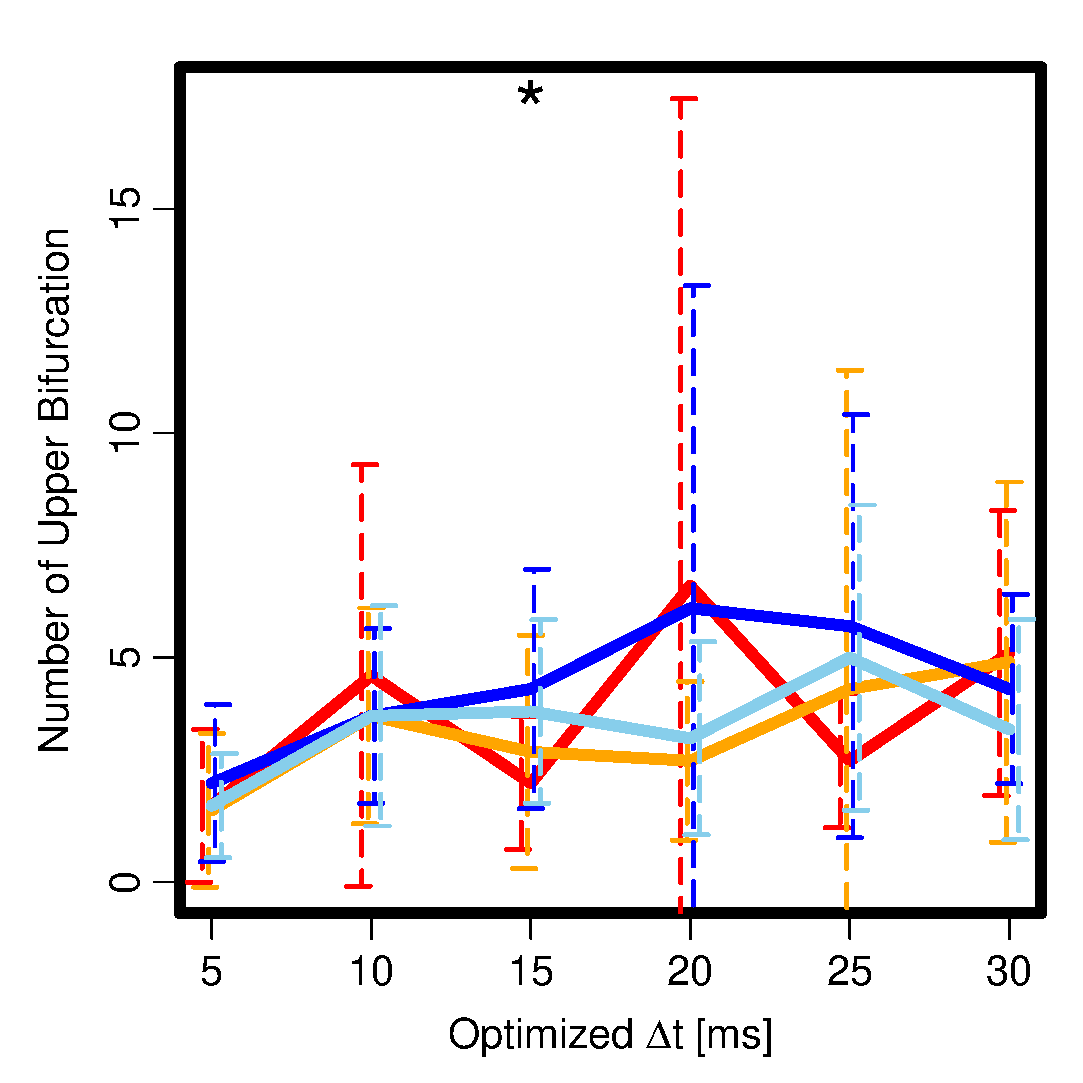
\includegraphics[width=0.8\columnwidth]{./Images_Result/k_ca_test_N_Upper_bif.eps}
         \caption{Upper Dend$B$NJ,4t?t(B}
         \label{k_ca_N_Upper_syn}
       \end{subfigure}

       \begin{subfigure}{0.5\columnwidth}
         \centering
         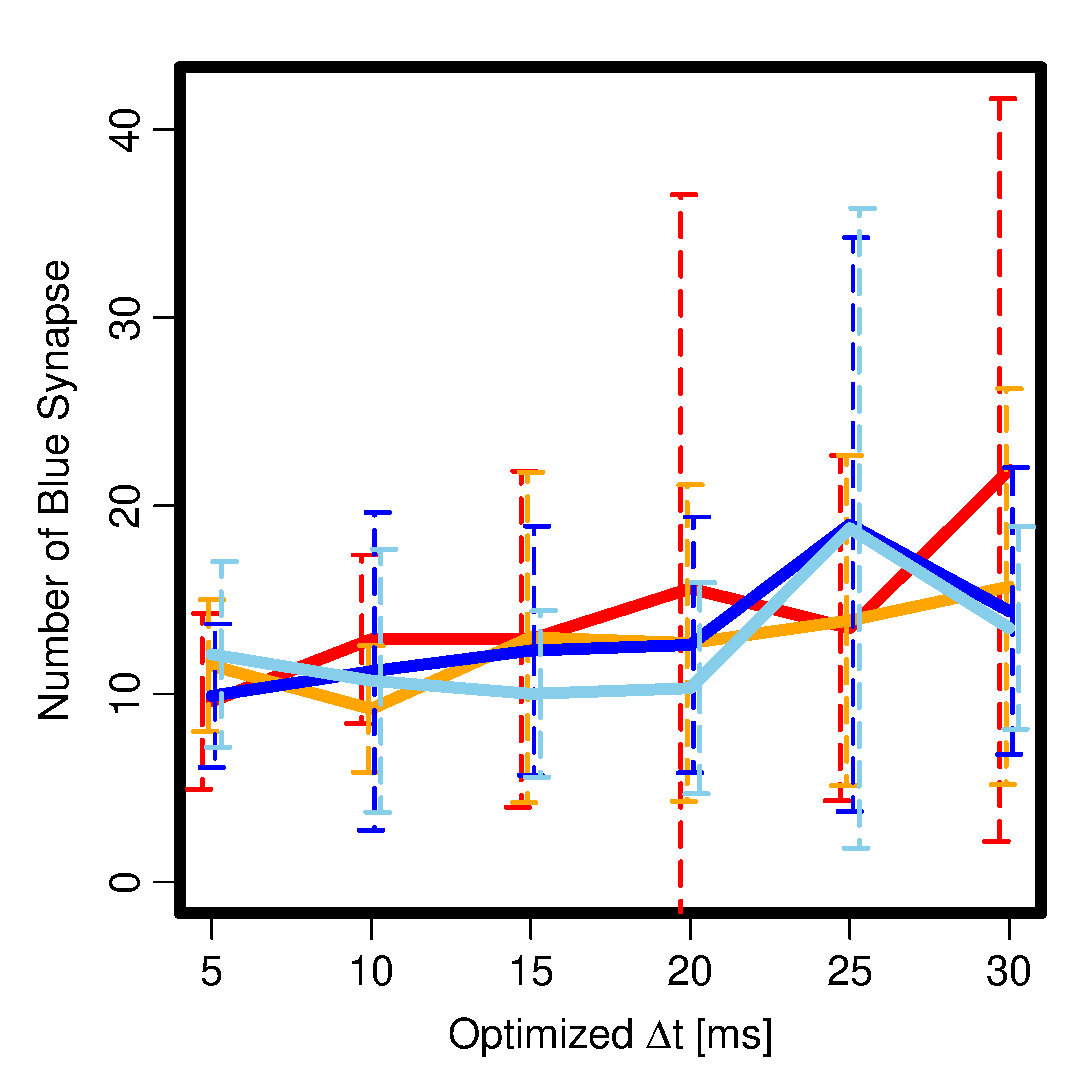
\includegraphics[width=0.8\columnwidth]{./Images_Result/k_ca_test_N_Lower_Syn.eps}
         \caption{Lower Dend$B$N%7%J%W%9?t(B}
         \label{k_ca_N_Lower_syn}
       \end{subfigure}
       \begin{subfigure}{0.5\columnwidth}
         \centering
         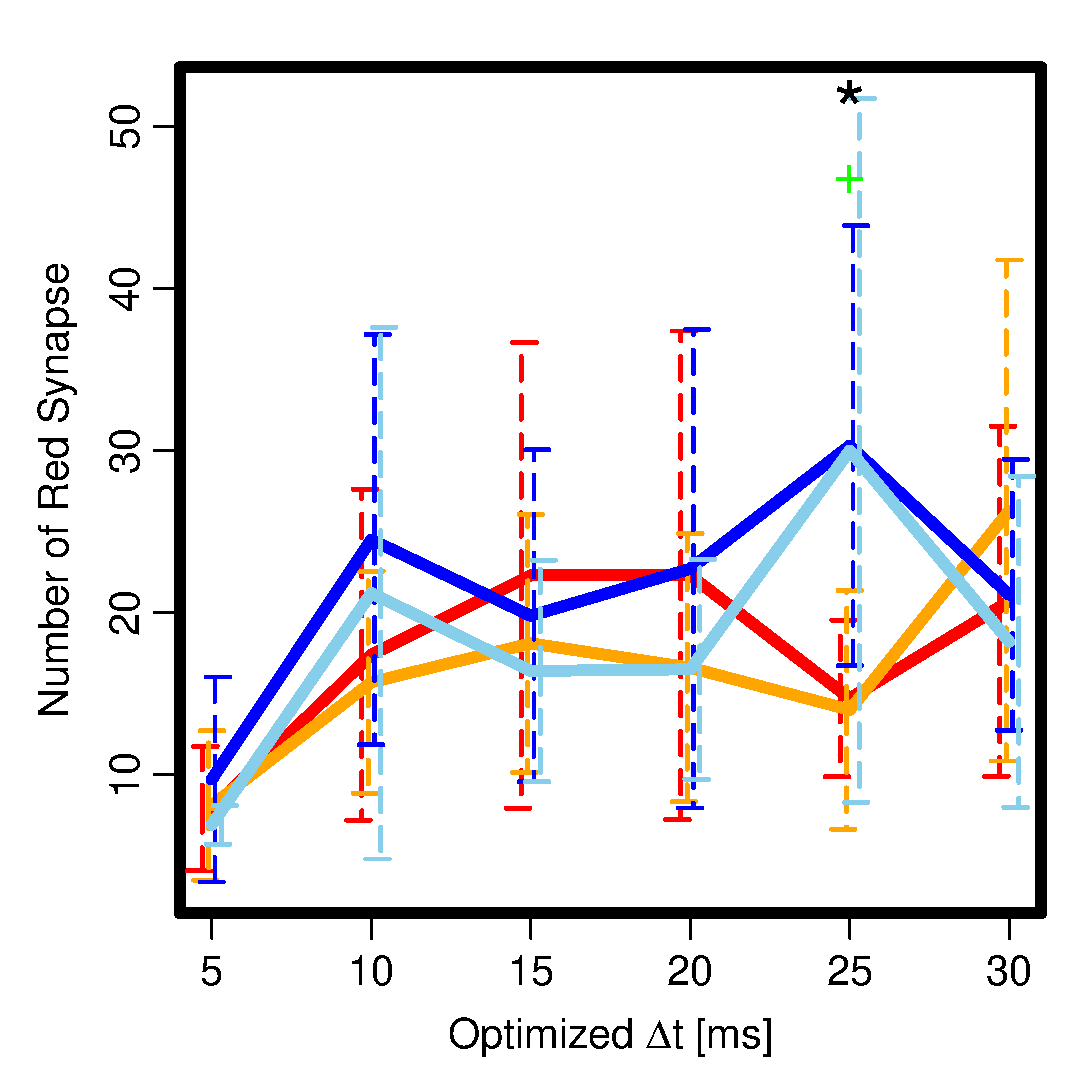
\includegraphics[width=0.8\columnwidth]{./Images_Result/k_ca_test_N_Upper_Syn.eps}
         \caption{Upper Dend$B$N%7%J%W%9?t(B}
         \label{k_ca_N_Upper_syn}
       \end{subfigure}


       \caption{Ka$B%A%c%M%k(B, CaT$B%A%c%M%k$rF3F~$7$?:]$N7k2L(B3} %$B%Z!<%8%l%$%"%&%H$,7hDj$7$F$+$iHyD4@0$9$k(B
       \label{k_ca_result3}
     \end{figure}

%$BIUO?$K$9$k(B
     %% $B0J2<$K(B${\Delta}t = 15$[ms]$B$G:n@.$7$??@7P:YK&$N(BKa$B%3%s%@%/%?%s%9(B
     %% $BJ,I[(B($B?^(B\ref{k_ca_K_dist_dt15}), CaT$B%3%s%@%/%?%s%9J,I[(B($B?^(B\ref{k_ca_Ca_dist_dt15})$B$r<($9(B.
     %% $B$^$?F1MM$K(B${\Delta}t = 30$[ms]$B$G:n@.$7$??@7P:YK&$N(BKa$B%3%s%@%/%?%s%9J,I[$r?^(B
     %% \ref{k_ca_K_dist_dt30}$B$K(B, CaT$B%3%s%@%/%?%s%9J,I[$r?^(B\ref{k_ca_Ca_dist_dt30}$B$K(B
     %% $B<($9(B. 
     %% %% \begin{figure}[H]
     %% %%   \begin{subfigure}{0.5\columnwidth}
     %% %%     \centering
     %% %%     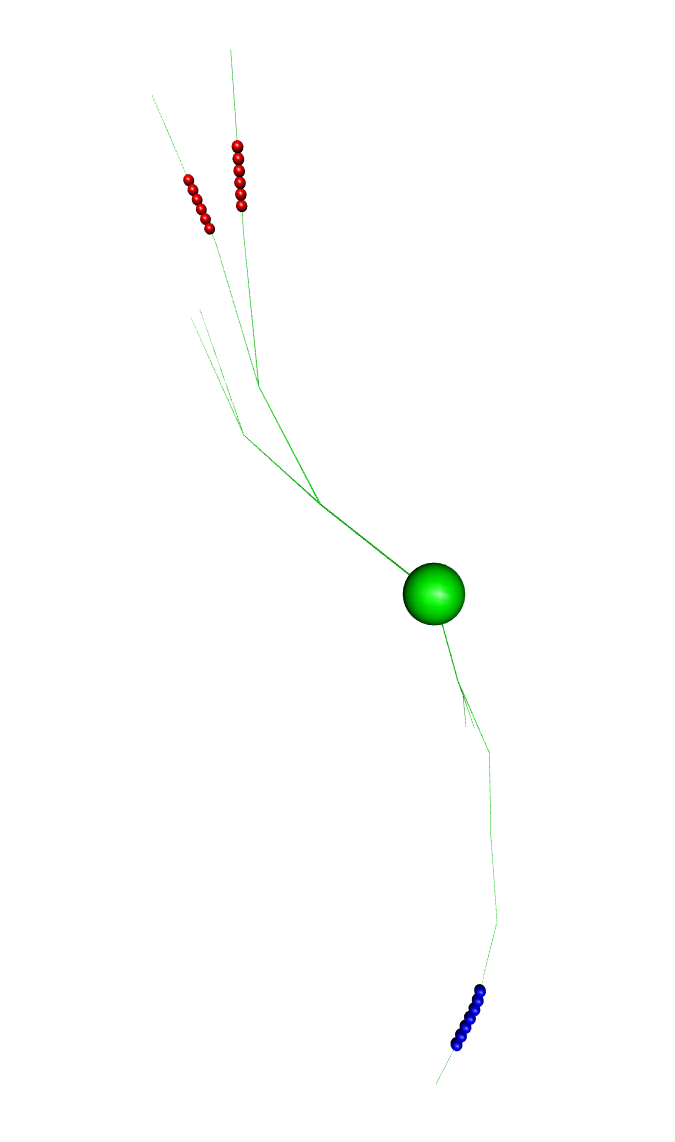
\includegraphics[width=0.8\columnwidth]{./Images_Result/k_ca_liner_TREE_sample_dt20_C5.png}
     %% %%     \caption{$B@~7AJ,I[(B}
     %% %%     \label{k_ca_liner_morpho}
     %% %%   \end{subfigure}
     %% %%          \begin{subfigure}{0.8\columnwidth}
     %% %%     \centering
     %% %%     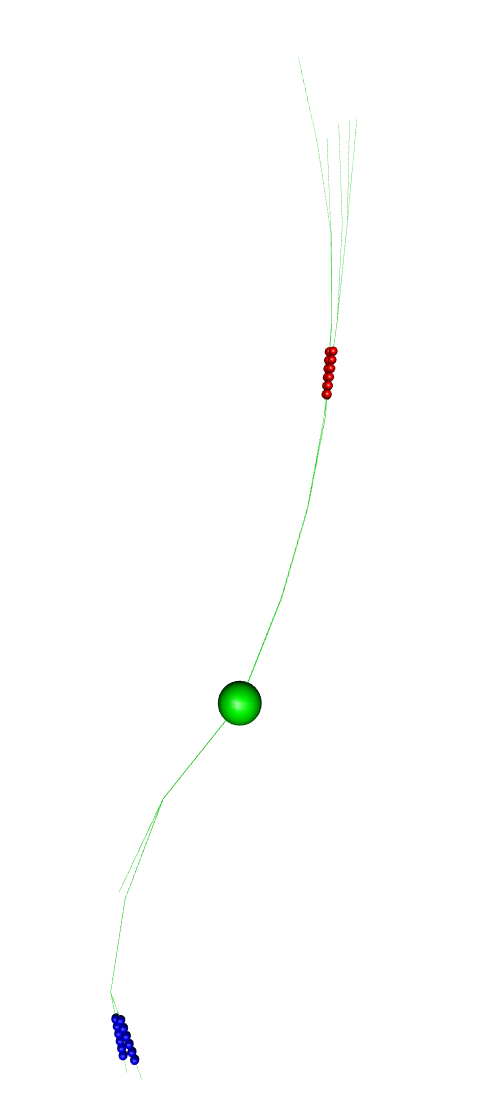
\includegraphics[width=0.8\columnwidth]{./Images_Result/k_ca_gaus_TREE_sample_dt20_C5.png}
     %% %%     \caption{$B%,%&%9J,I[(B}
     %% %%     \label{k_ca_gaus_morpho}
     %% %%   \end{subfigure}

     %% %%   \caption{Ka$B%A%c%M%k(B, CaT$B%A%c%M%k$rF3F~$7$?:]$N7k2L(B1} %$B%Z!<%8%l%$%"%&%H$,7hDj$7$F$+$iHyD4@0$9$k(B
     %% %%   \label{k_ca_morpho}
     %% %% \end{figure}

     %% \begin{figure}[H]
     %%   \hspace*{-2cm}
     %%   \begin{subfigure}{0.62\columnwidth}
     %%     \centering
     %%     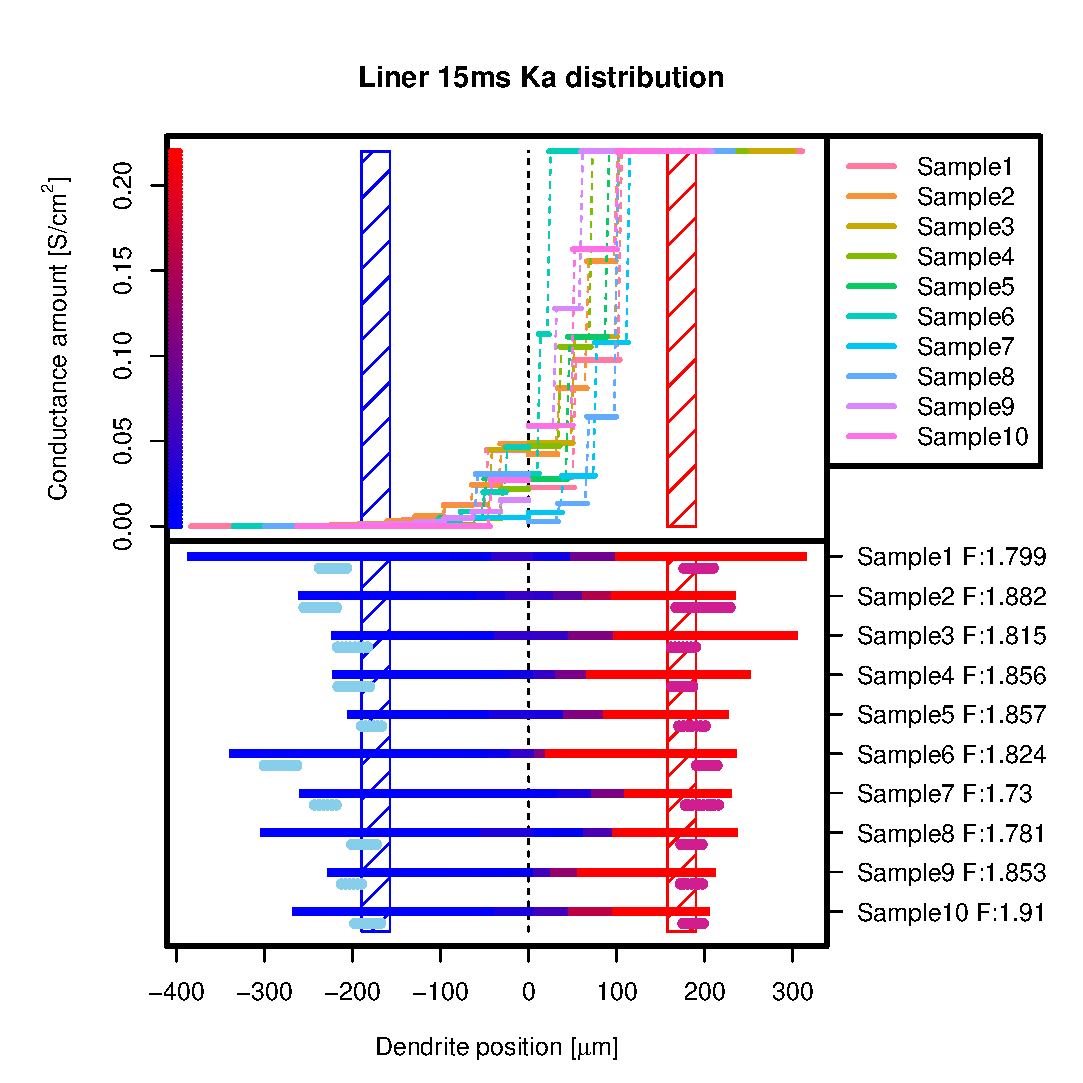
\includegraphics[width=\columnwidth]{./Images_Result/k_ca_Rerative_liner_75_0_K_distribution_dt15.eps}
     %%     \caption{$B@~7AJ,I[(B}
     %%     \label{k_ca_K_liner_reduced_dist}
     %%   \end{subfigure}
     %%   \begin{subfigure}{0.62\columnwidth}
     %%     \centering
     %%     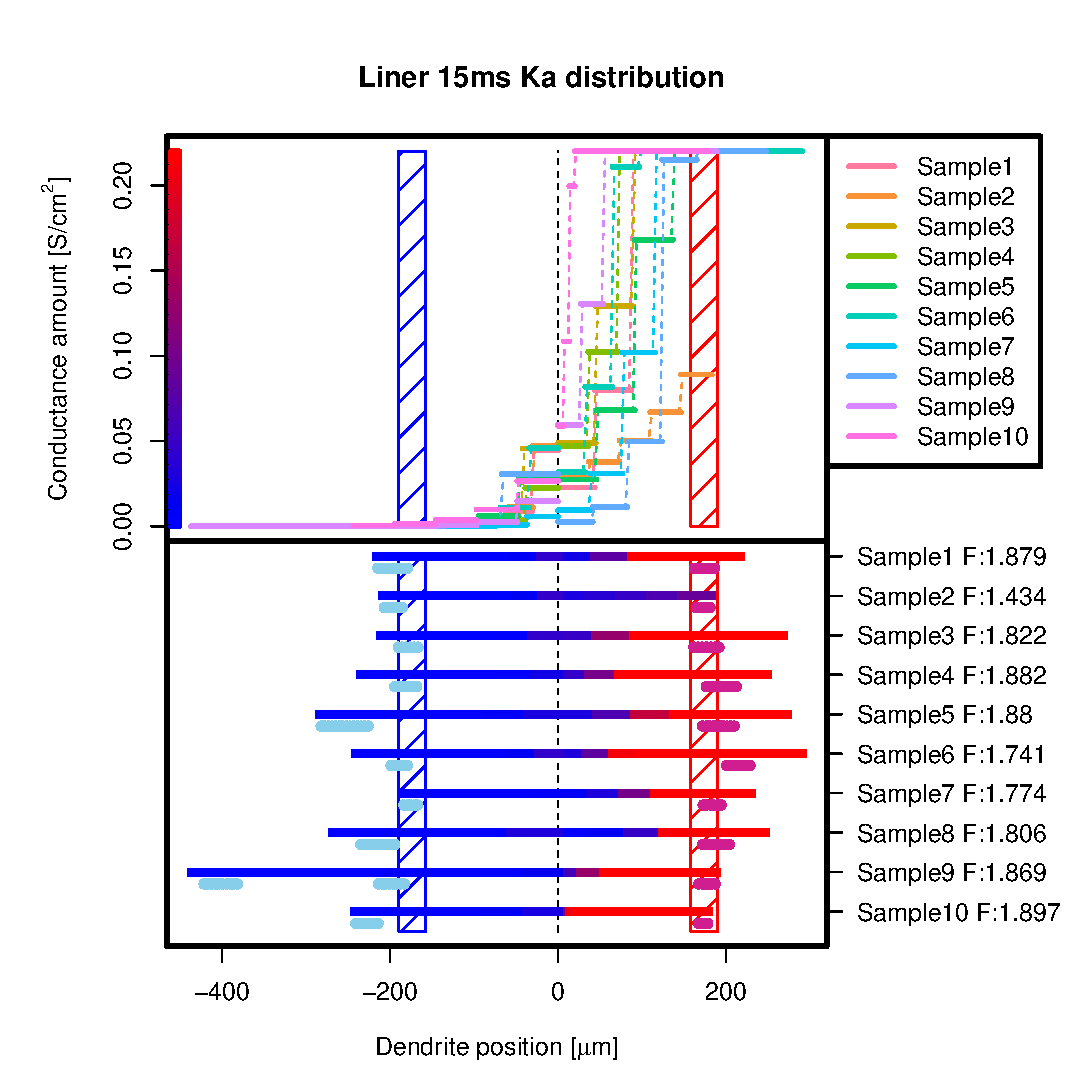
\includegraphics[width=\columnwidth]{./Images_Result/k_ca_Rerative_liner_75_5_K_distribution_dt15.eps}
     %%     \caption{$B@~7AJ,I[(B(reduced)}
     %%     \label{k_ca_K_liner_reduced_dist}
     %%   \end{subfigure}

     %%   \vspace{-1.5cm}
     %%   \begin{subfigure}{\columnwidth}
     %%     \centering
     %%     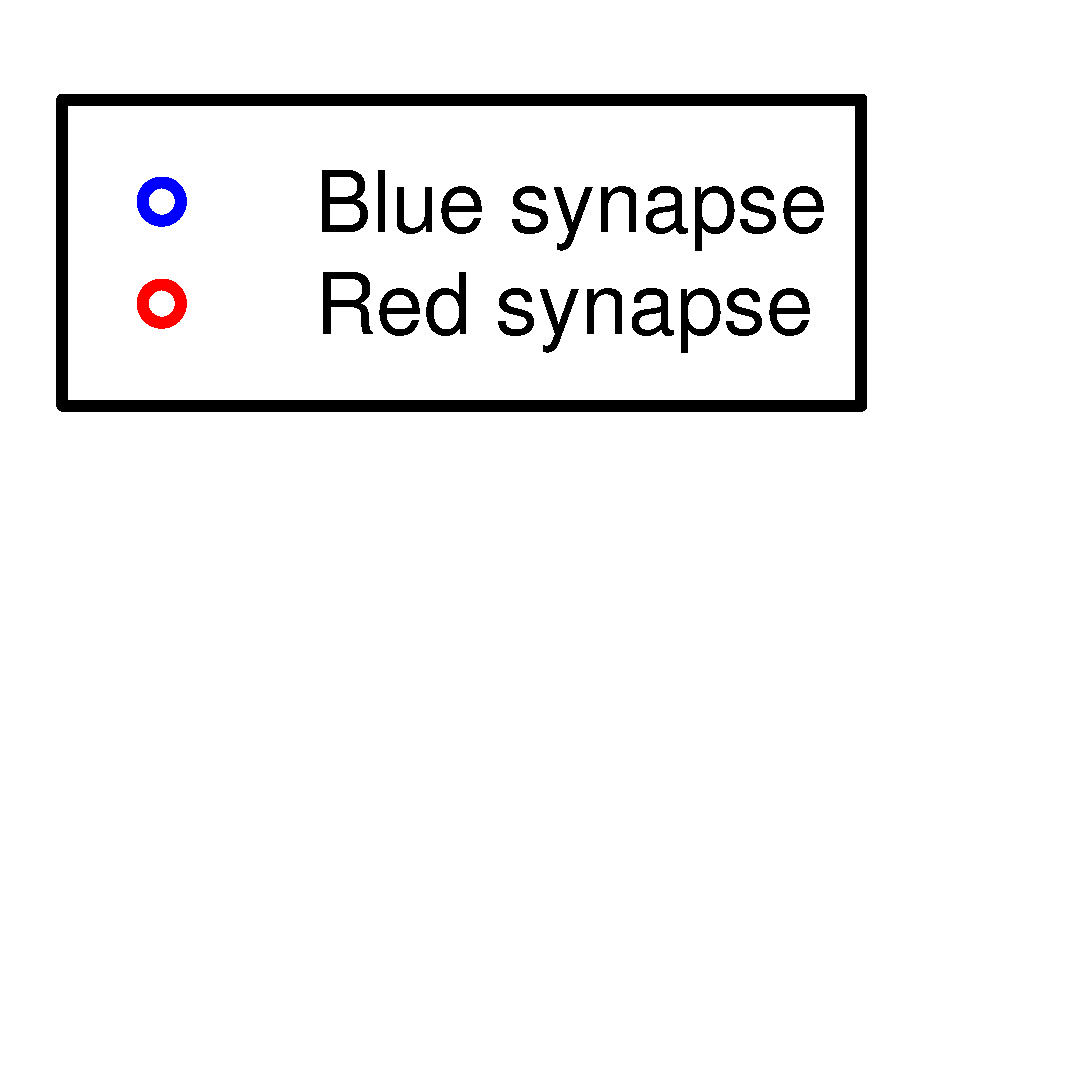
\includegraphics[width=0.35\columnwidth]{./Images_Result/Synapse_legend.eps} 
     %%   \end{subfigure}
     %%   \vspace{-4cm}

     %%   \hspace*{-2cm}
     %%   \begin{subfigure}{0.62\columnwidth}
     %%     \centering
     %%     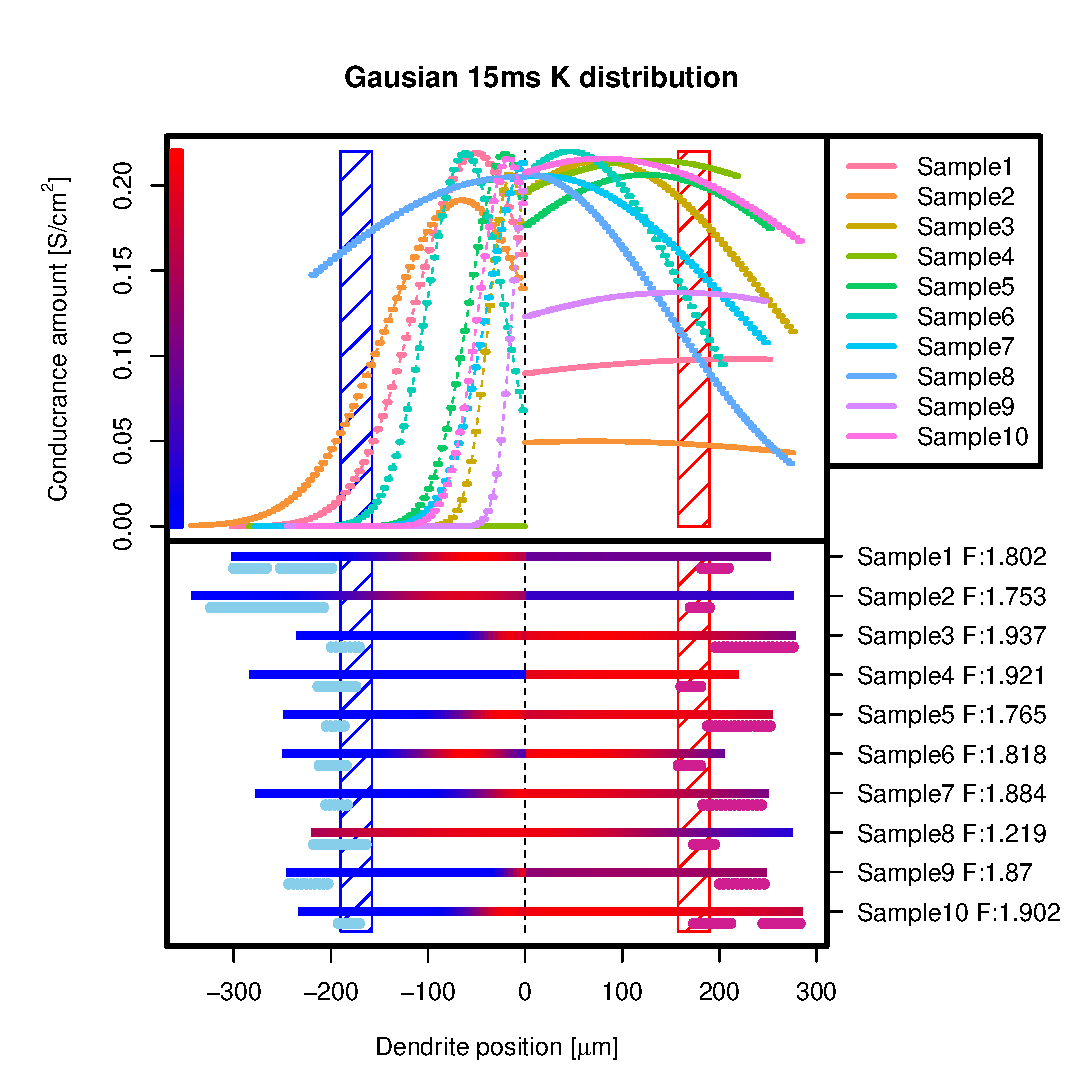
\includegraphics[width=\columnwidth]{./Images_Result/k_ca_Rerative_Gaus_75_0_K_distribution_dt15.eps}
     %%     \caption{$B%,%&%9J,I[(B}
     %%     \label{k_ca_K_gaus_reduced_dist}
     %%   \end{subfigure}
     %%   \begin{subfigure}{0.62\columnwidth}
     %%     \centering
     %%     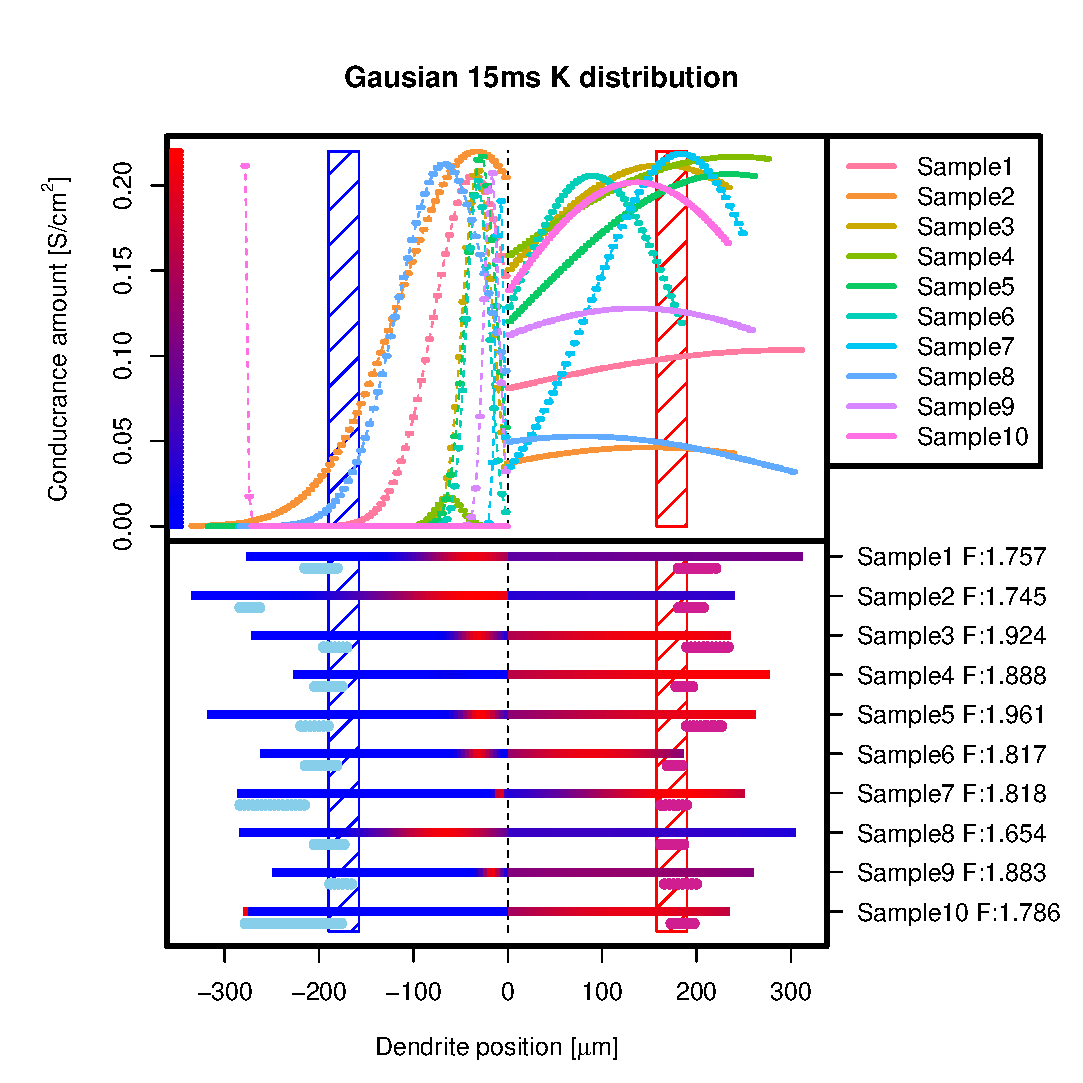
\includegraphics[width=\columnwidth]{./Images_Result/k_ca_Rerative_Gaus_75_5_K_distribution_dt15.eps}
     %%     \caption{$B%,%&%9J,I[(B(reduced)}
     %%     \label{k_ca_K_gaus_reduced_dist}
     %%   \end{subfigure}
       
     %%   \caption{${\Delta}t = 15$[ms]$B$G$N(BKa$B%3%s%@%/%?%s%9J,I[(B}
     %%   \label{k_ca_K_dist_dt15}
     %% \end{figure}

     %% \begin{figure}[H]
     %%   \hspace*{-2cm}
     %%   \begin{subfigure}{0.62\columnwidth}
     %%     \centering
     %%     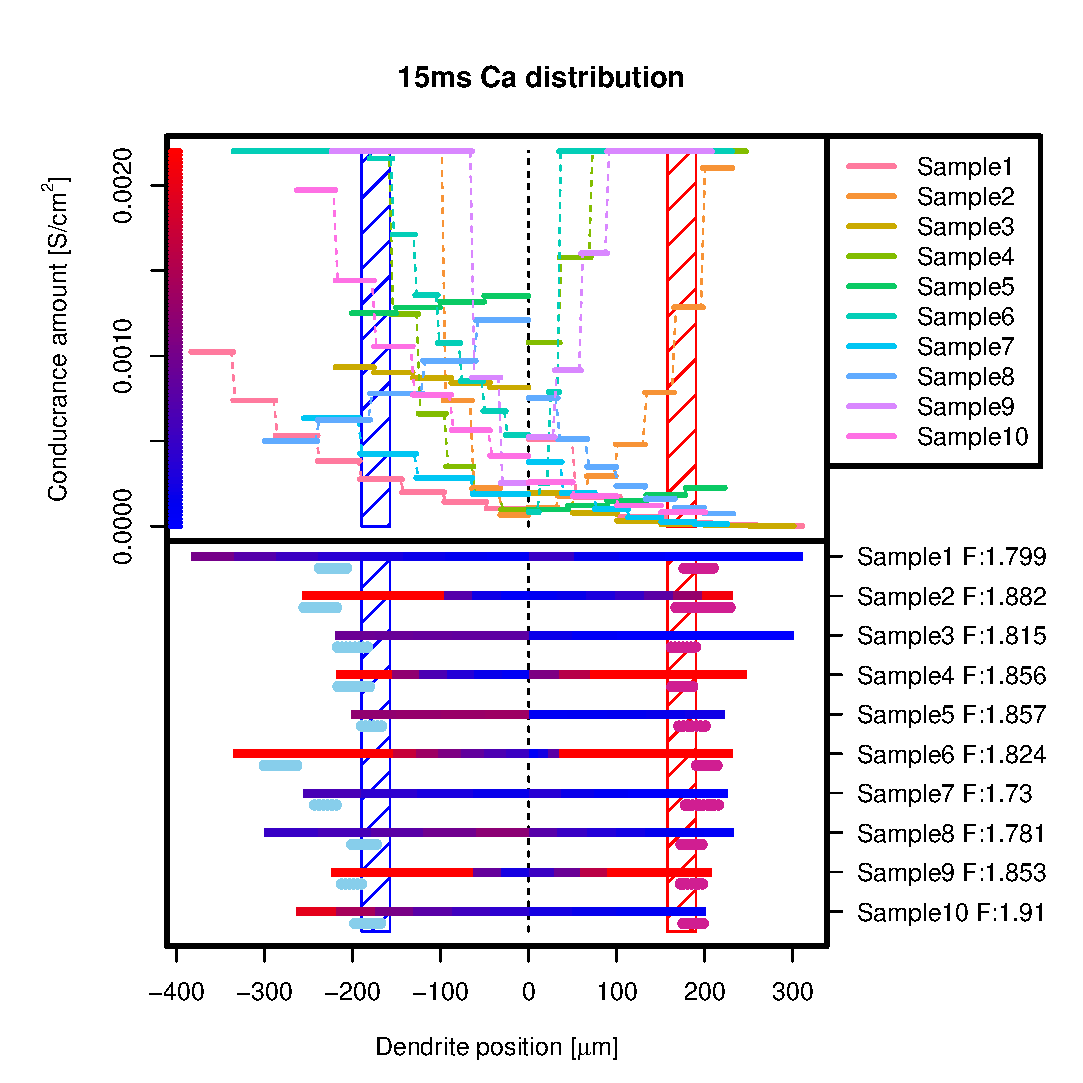
\includegraphics[width=\columnwidth]{./Images_Result/k_ca_Rerative_liner_75_0_Ca_distribution_dt15.eps}
     %%     \caption{$B@~7AJ,I[(B}
     %%     \label{k_ca_Ca_liner_reduced_dist}
     %%   \end{subfigure}
     %%   \begin{subfigure}{0.62\columnwidth}
     %%     \centering
     %%     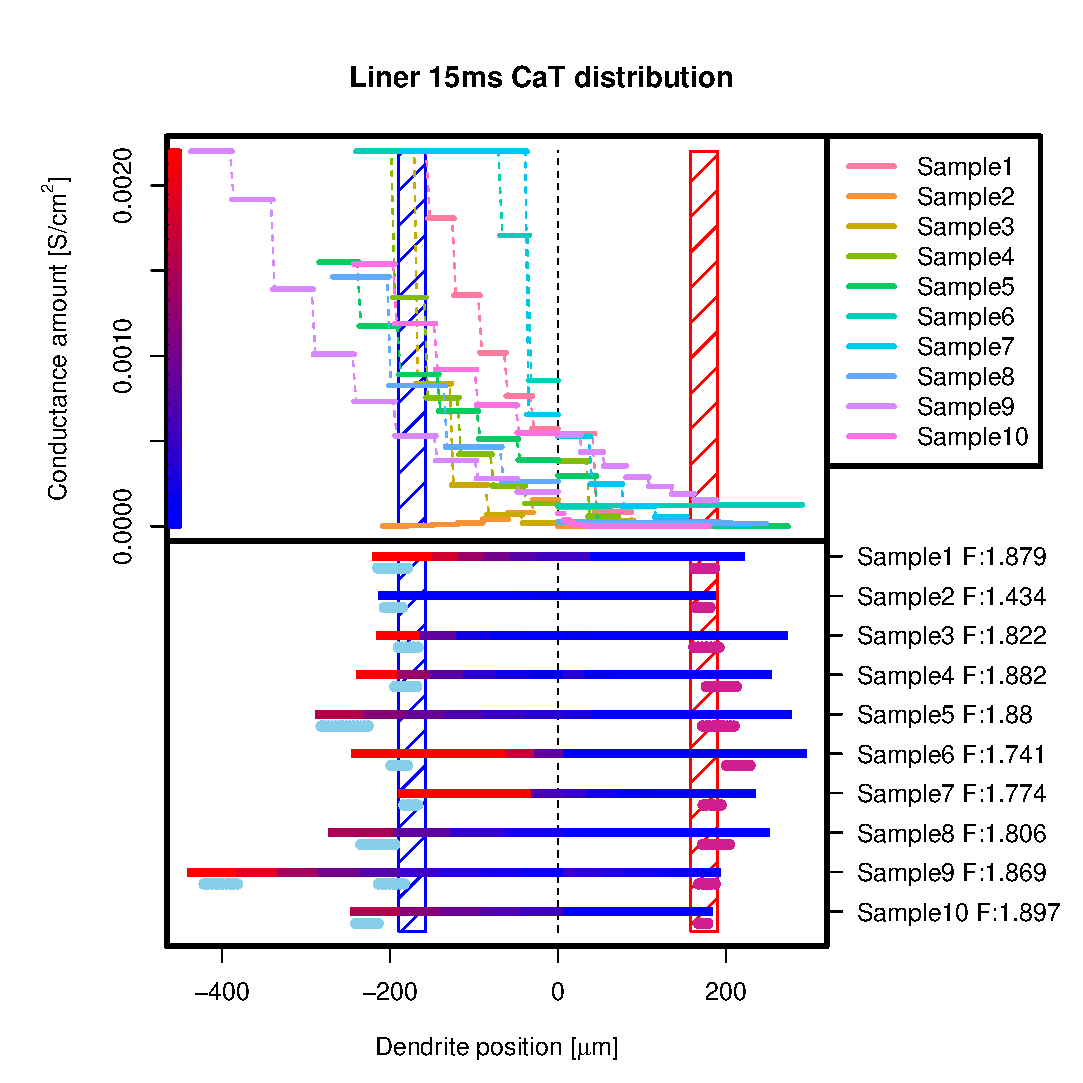
\includegraphics[width=\columnwidth]{./Images_Result/k_ca_Rerative_liner_75_5_Ca_distribution_dt15.eps}
     %%     \caption{$B@~7AJ,I[(B(reduced)}
     %%     \label{k_ca_Ca_liner_reduced_dist}
     %%   \end{subfigure}

     %%   \vspace{-1.5cm}
     %%   \begin{subfigure}{\columnwidth}
     %%     \centering
     %%     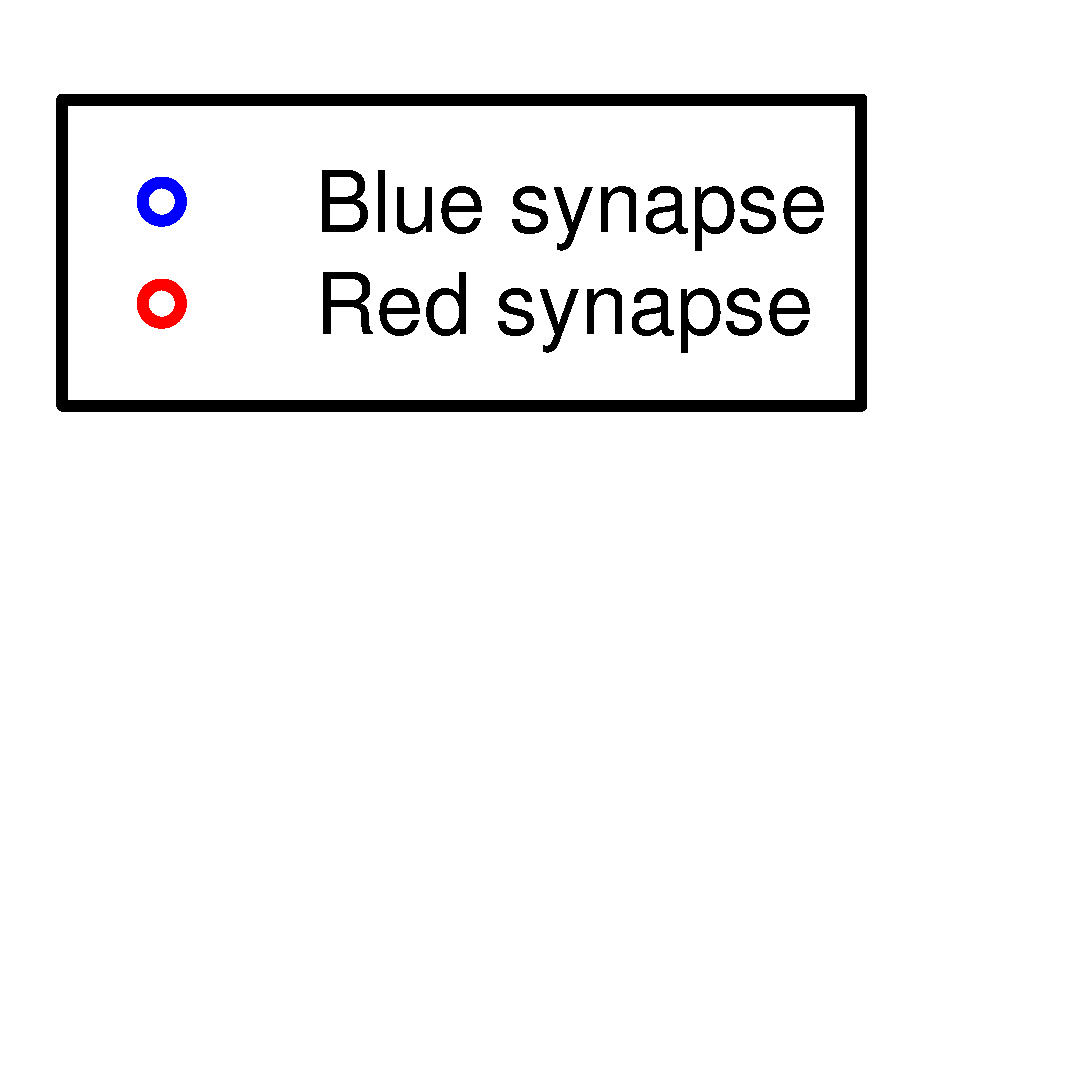
\includegraphics[width=0.35\columnwidth]{./Images_Result/Synapse_legend.eps} 
     %%   \end{subfigure}
     %%   \vspace{-4cm}

     %%   \hspace*{-2cm}
     %%   \begin{subfigure}{0.62\columnwidth}
     %%     \centering
     %%     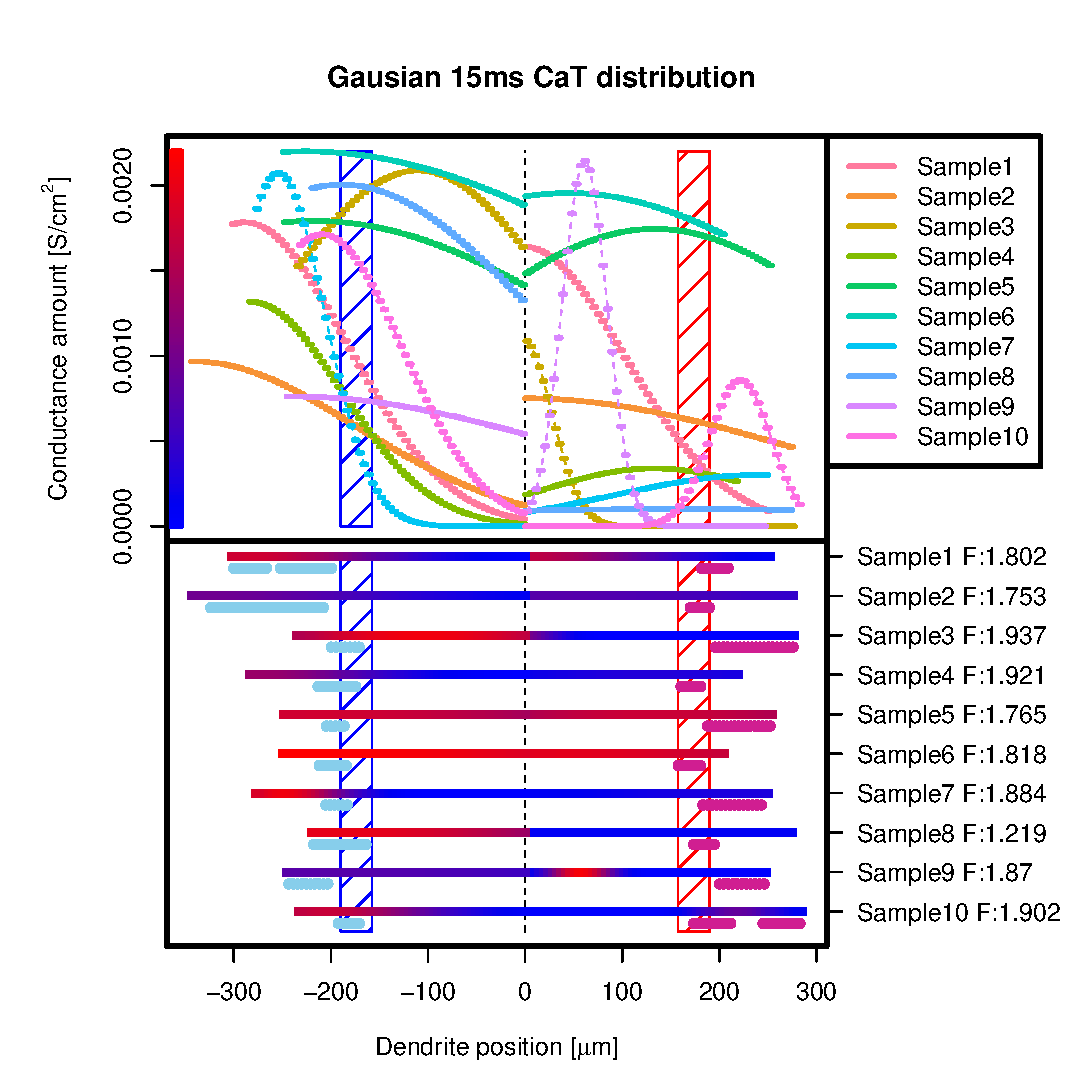
\includegraphics[width=\columnwidth]{./Images_Result/k_ca_Rerative_Gaus_75_0_Ca_distribution_dt15.eps}
     %%     \caption{$B%,%&%9J,I[(B}
     %%     \label{k_ca_Ca_gaus_reduced_dist}
     %%   \end{subfigure}
     %%   \begin{subfigure}{0.62\columnwidth}
     %%     \centering
     %%     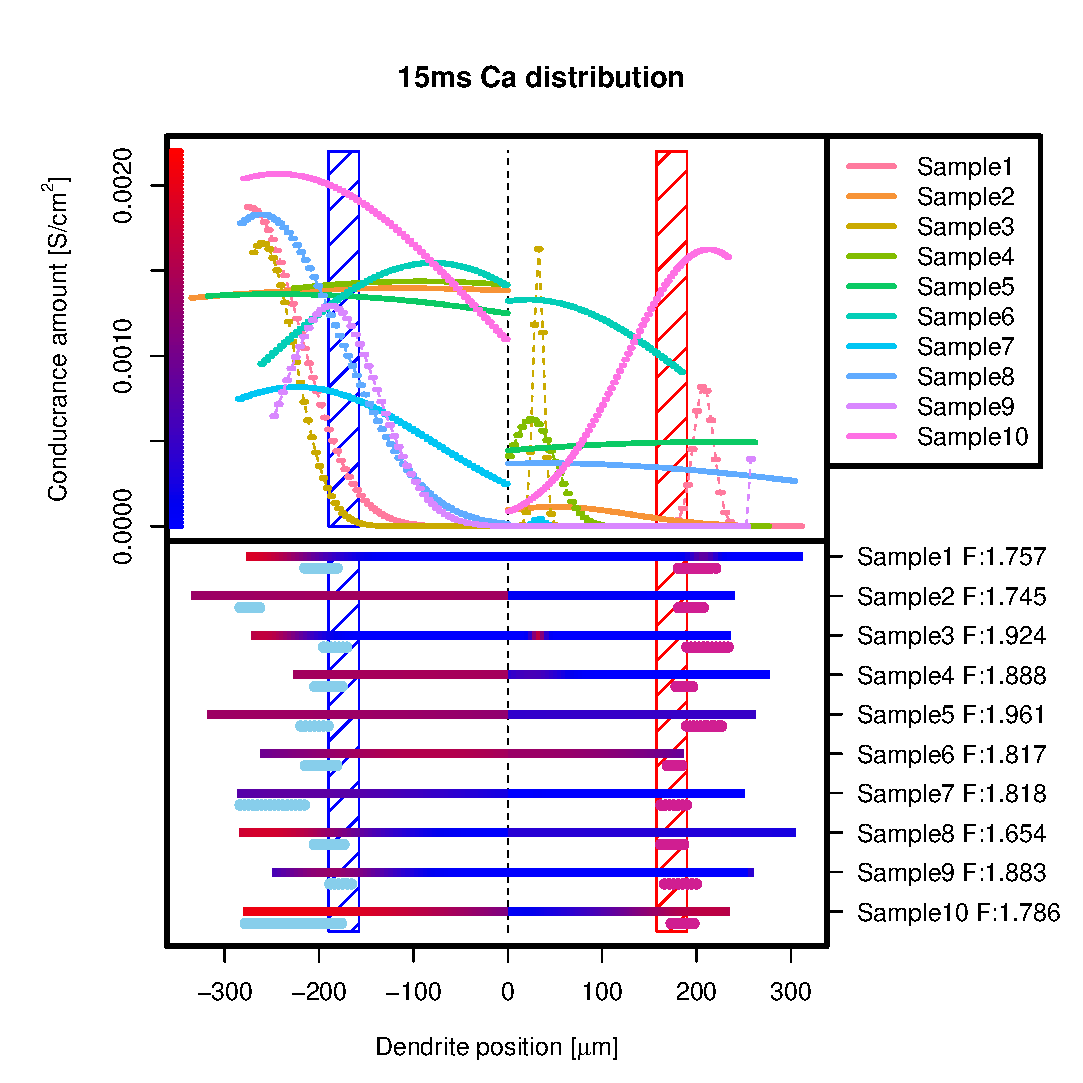
\includegraphics[width=\columnwidth]{./Images_Result/k_ca_Rerative_Gaus_75_5_Ca_distribution_dt15.eps}
     %%     \caption{$B%,%&%9J,I[(B(reduced)}
     %%     \label{k_ca_Ca_gaus_reduced_dist}
     %%   \end{subfigure}

     %%   \caption{${\Delta}t = 15$[ms]$B$G$N(BCaT$B%3%s%@%/%?%s%9J,I[(B}
     %%   \label{k_ca_Ca_dist_dt15}
     %% \end{figure}

     %% %------------------------------------------------------------

     %% \begin{figure}[H]
     %%   \hspace*{-2cm}
     %%   \begin{subfigure}{0.62\columnwidth}
     %%     \centering
     %%     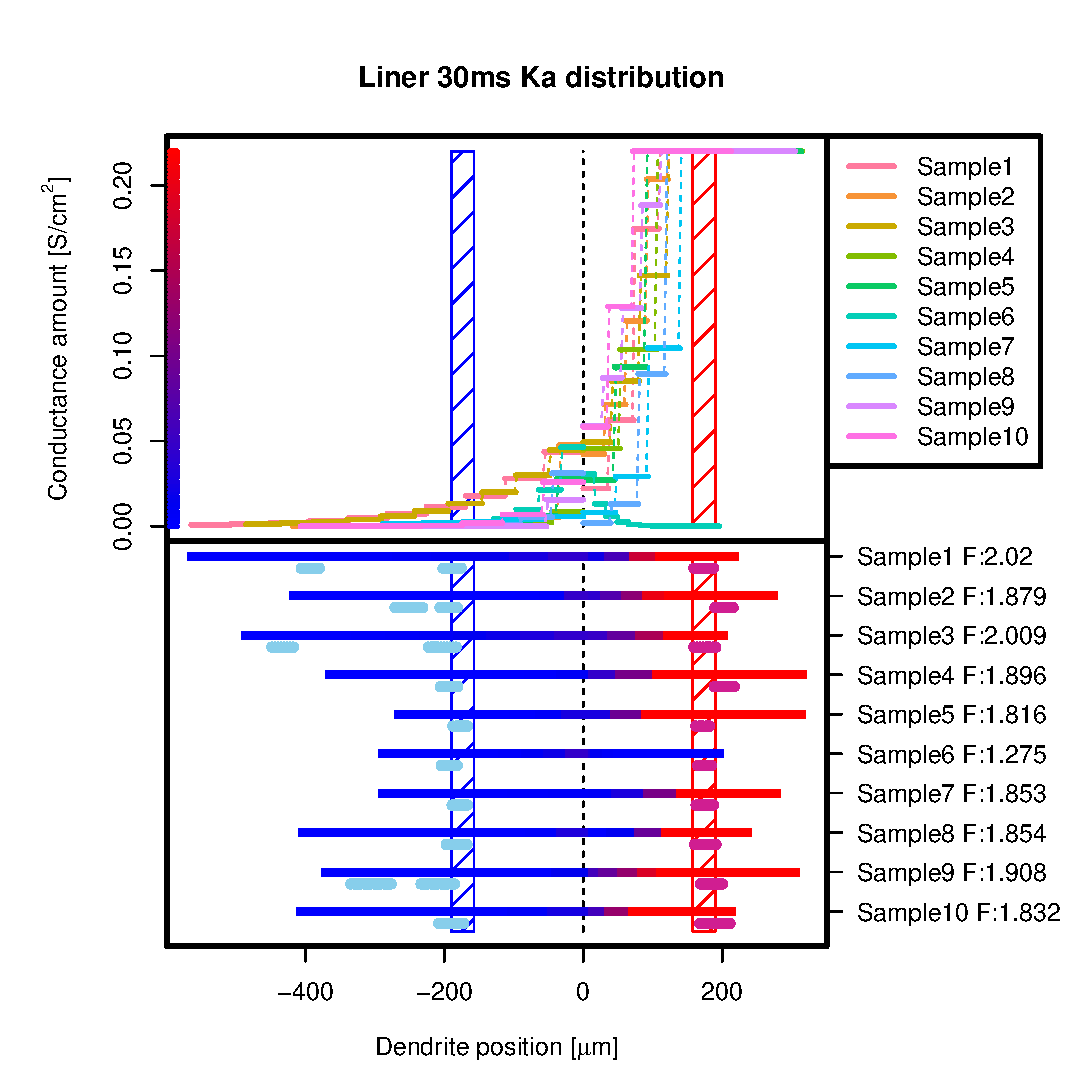
\includegraphics[width=\columnwidth]{./Images_Result/k_ca_Rerative_liner_75_0_K_distribution_dt30.eps}
     %%     \caption{$B@~7AJ,I[(B}
     %%     \label{k_ca_K_liner_reduced_dist}
     %%   \end{subfigure}
     %%   \begin{subfigure}{0.62\columnwidth}
     %%     \centering
     %%     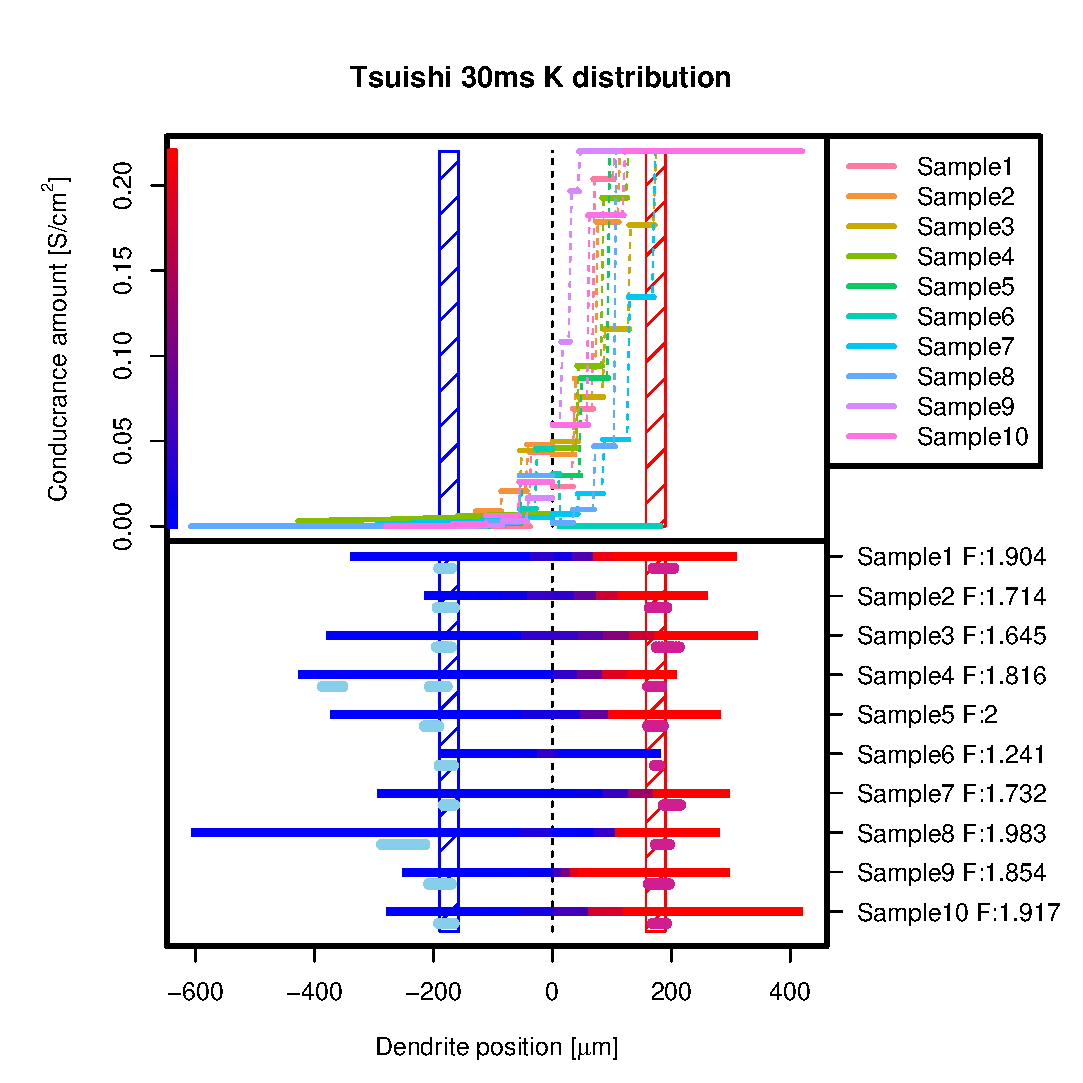
\includegraphics[width=\columnwidth]{./Images_Result/k_ca_Rerative_liner_75_5_K_distribution_dt30.eps}
     %%     \caption{$B@~7AJ,I[(B(reduced)}
     %%     \label{k_ca_K_liner_reduced_dist}
     %%   \end{subfigure}

     %%   \vspace{-1.5cm}
     %%   \begin{subfigure}{\columnwidth}
     %%     \centering
     %%     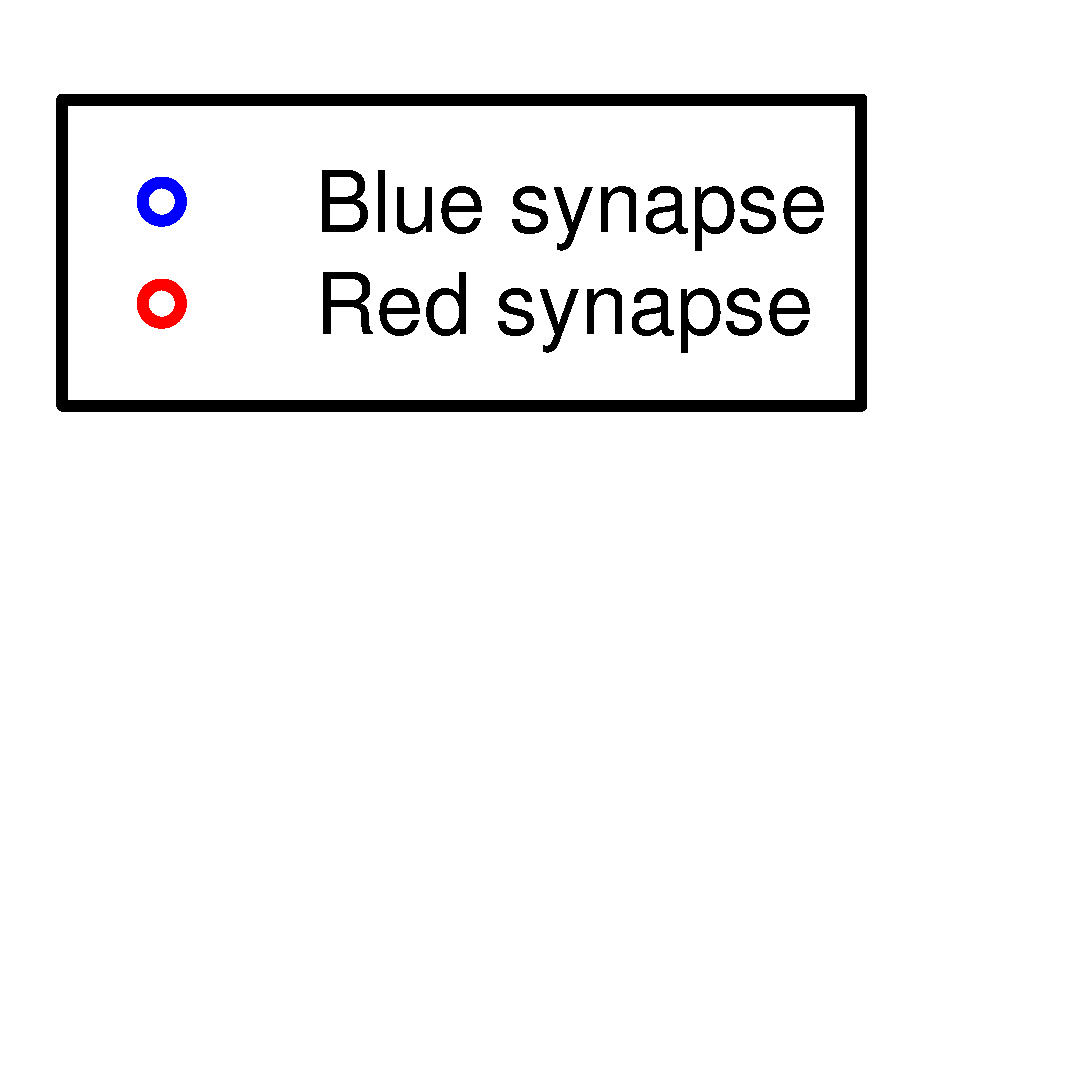
\includegraphics[width=0.35\columnwidth]{./Images_Result/Synapse_legend.eps} 
     %%   \end{subfigure}
     %%   \vspace{-4cm}

     %%   \hspace*{-2cm}
     %%   \begin{subfigure}{0.62\columnwidth}
     %%     \centering
     %%     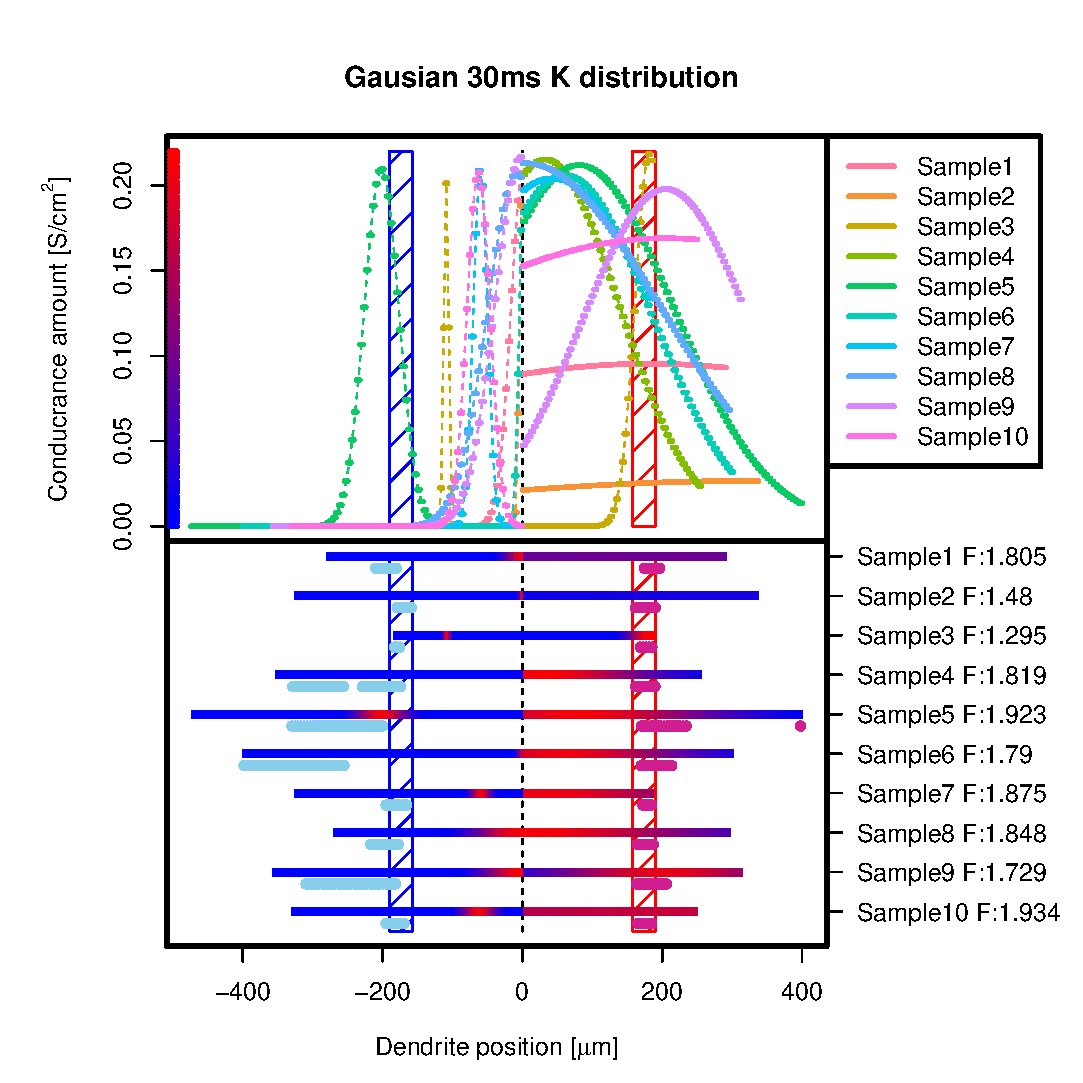
\includegraphics[width=\columnwidth]{./Images_Result/k_ca_Rerative_Gaus_75_0_K_distribution_dt30.eps}
     %%     \caption{$B%,%&%9J,I[(B}
     %%     \label{k_ca_K_gaus_reduced_dist}
     %%   \end{subfigure}
     %%   \begin{subfigure}{0.62\columnwidth}
     %%     \centering
     %%     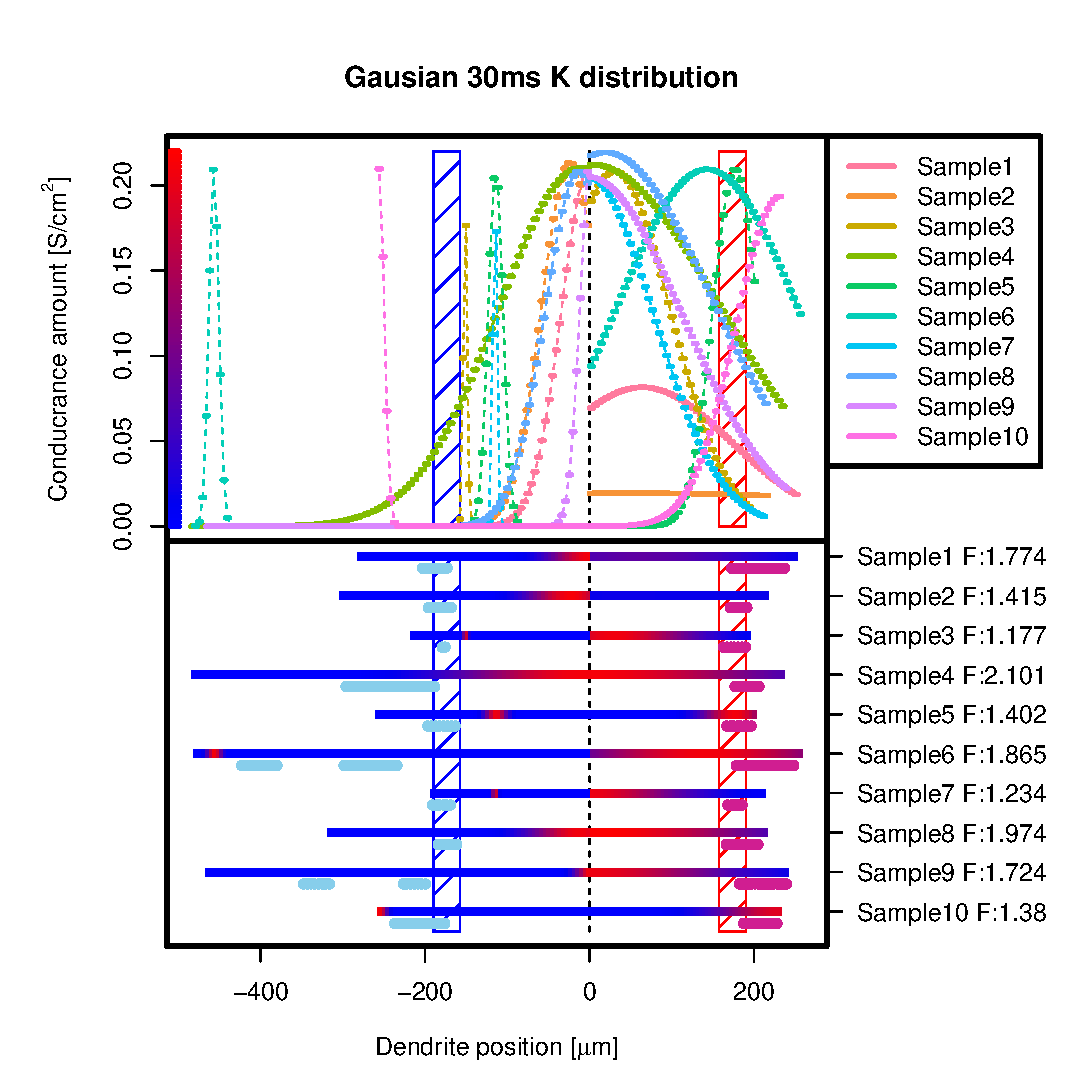
\includegraphics[width=\columnwidth]{./Images_Result/k_ca_Rerative_Gaus_75_5_K_distribution_dt30.eps}
     %%     \caption{$B%,%&%9J,I[(B(reduced)}
     %%     \label{k_ca_K_gaus_reduced_dist}
     %%   \end{subfigure}

     %%   \caption{${\Delta}t = 30$[ms]$B$G$N(BKa$B%3%s%@%/%?%s%9J,I[(B}
     %%   \label{k_ca_K_dist_dt30}
     %% \end{figure}

     %% \begin{figure}[H]
     %%   \hspace*{-2cm}
     %%   \begin{subfigure}{0.62\columnwidth}
     %%     \centering
     %%     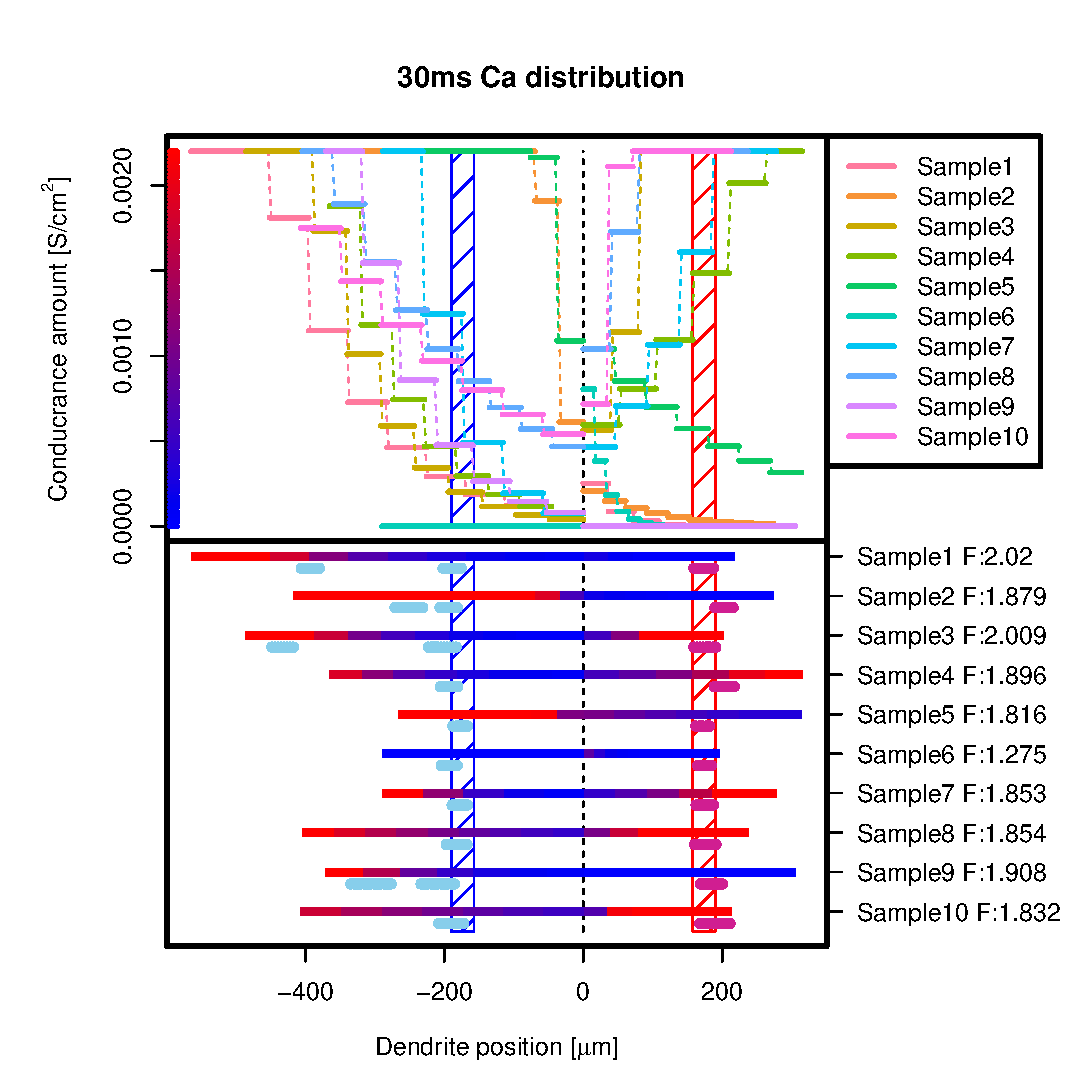
\includegraphics[width=\columnwidth]{./Images_Result/k_ca_Rerative_liner_75_0_Ca_distribution_dt30.eps}
     %%     \caption{$B@~7AJ,I[(B}
     %%     \label{k_ca_Ca_liner_reduced_dist}
     %%   \end{subfigure}
     %%   \begin{subfigure}{0.62\columnwidth}
     %%     \centering
     %%     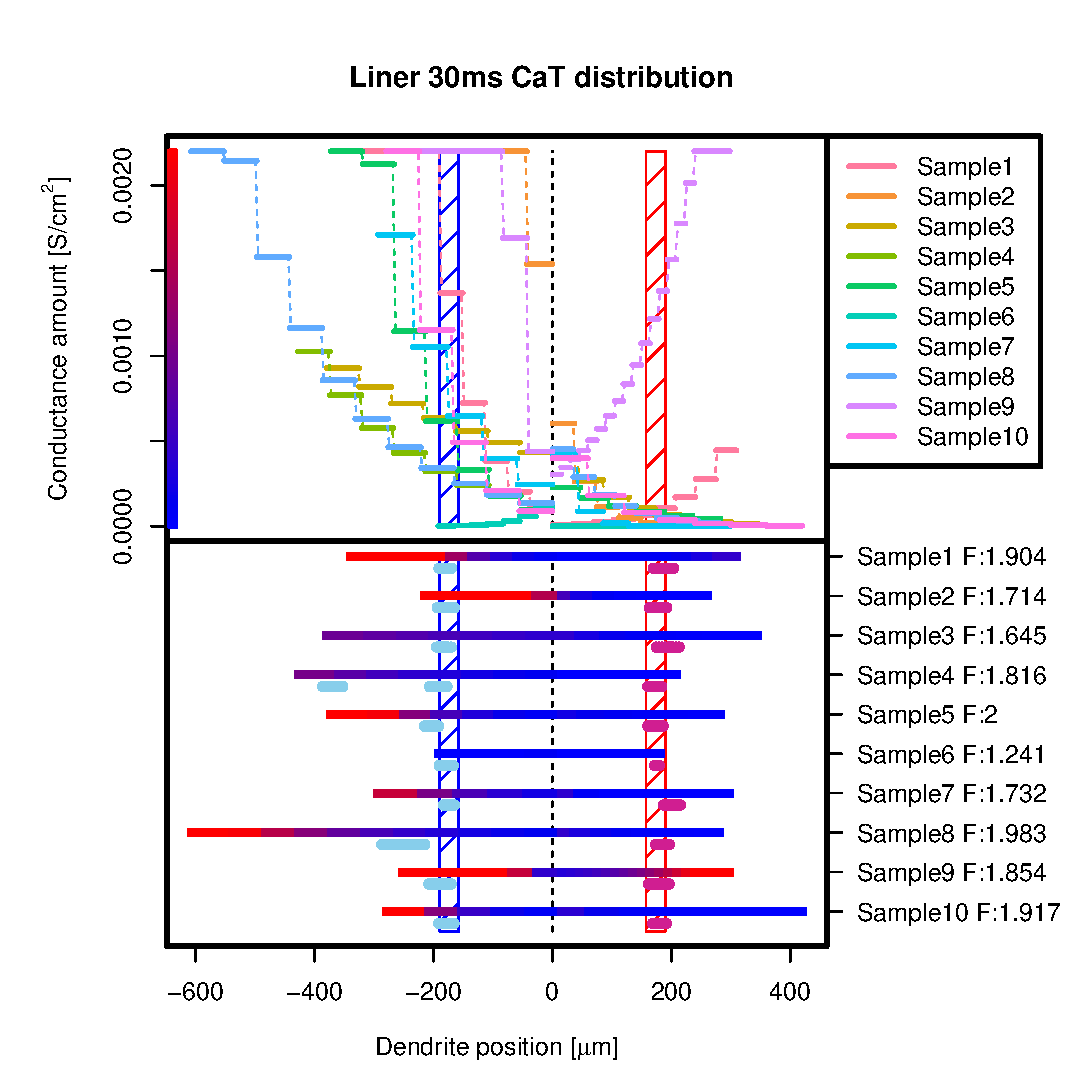
\includegraphics[width=\columnwidth]{./Images_Result/k_ca_Rerative_liner_75_5_Ca_distribution_dt30.eps}
     %%     \caption{$B@~7AJ,I[(B(reduced)}
     %%     \label{k_ca_Ca_liner_reduced_dist}
     %%   \end{subfigure}

     %%   \vspace{-1.5cm}
     %%   \begin{subfigure}{\columnwidth}
     %%     \centering
     %%     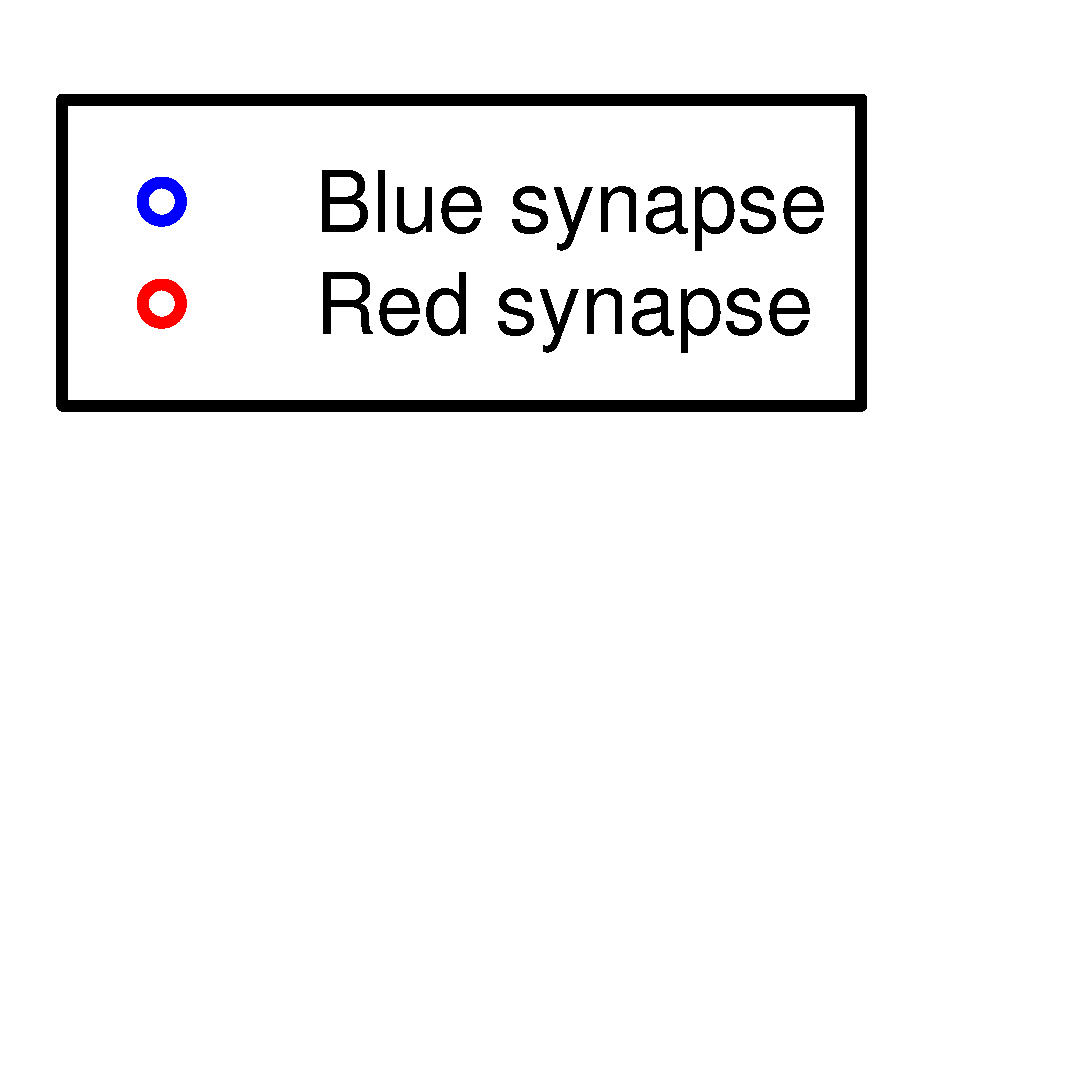
\includegraphics[width=0.35\columnwidth]{./Images_Result/Synapse_legend.eps} 
     %%   \end{subfigure}
     %%   \vspace{-4cm}

     %%   \hspace*{-2cm}
     %%   \begin{subfigure}{0.62\columnwidth}
     %%     \centering
     %%     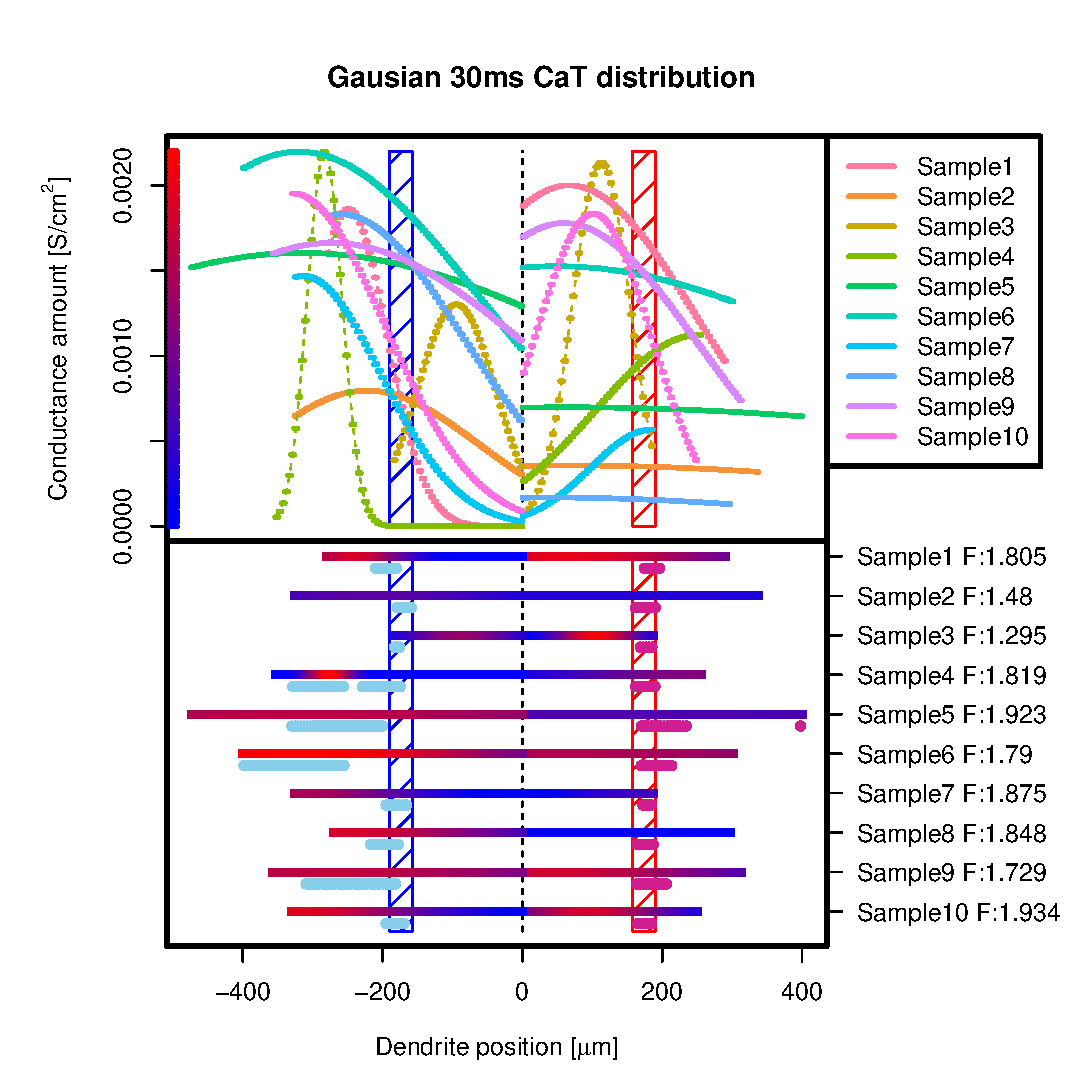
\includegraphics[width=\columnwidth]{./Images_Result/k_ca_Rerative_Gaus_75_0_Ca_distribution_dt30.eps}
     %%     \caption{$B%,%&%9J,I[(B}
     %%     \label{k_ca_Ca_gaus_reduced_dist}
     %%   \end{subfigure}
     %%   \begin{subfigure}{0.62\columnwidth}
     %%     \centering
     %%     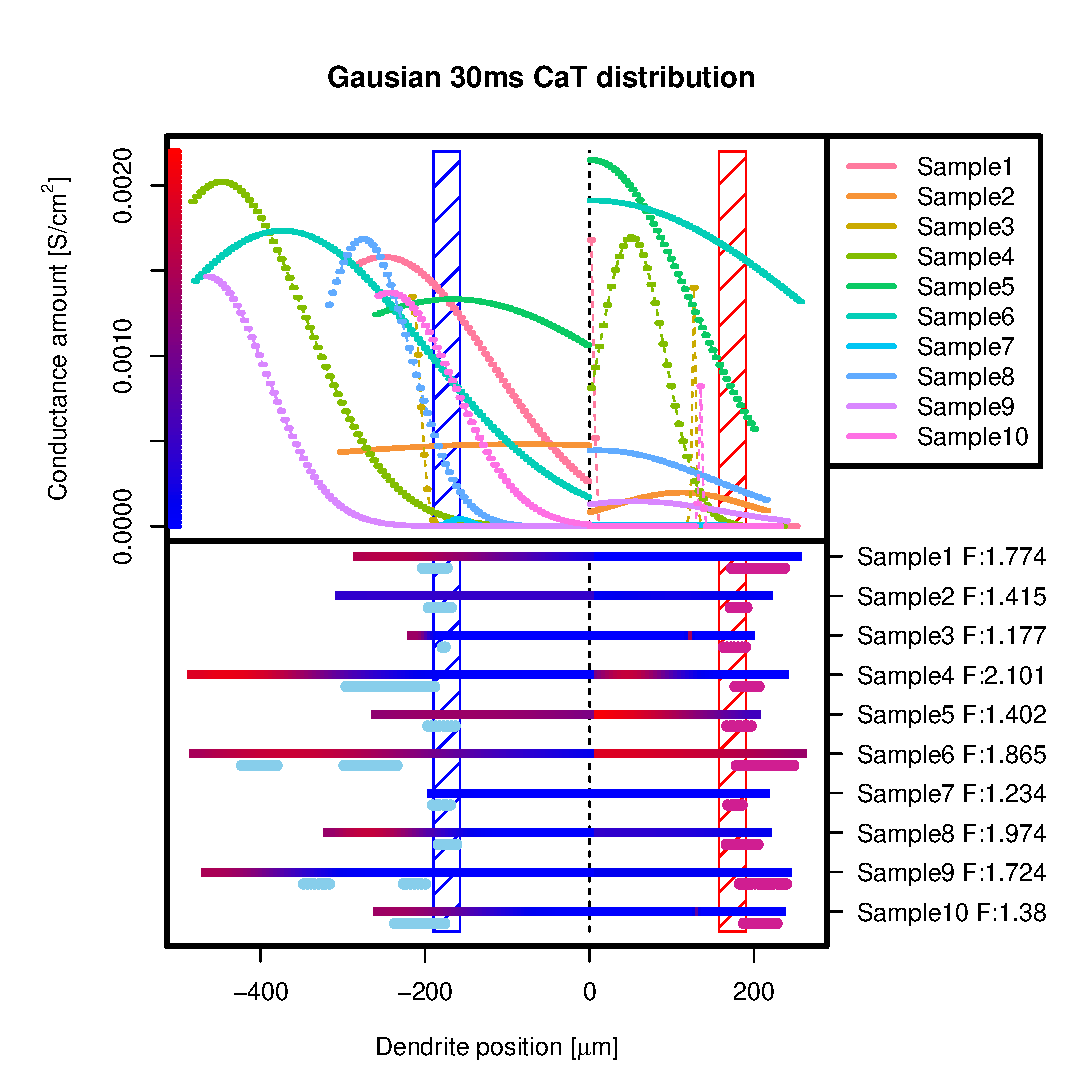
\includegraphics[width=\columnwidth]{./Images_Result/k_ca_Rerative_Gaus_75_5_Ca_distribution_dt30.eps}
     %%     \caption{$B%,%&%9J,I[(B(reduced)}
     %%     \label{k_ca_Ca_gaus_reduced_dist}
     %%   \end{subfigure}
       
     %%   \caption{${\Delta}t = 30$[ms]$B$G$N(BCaT$B%3%s%@%/%?%s%9J,I[(B}
     %%   \label{k_ca_Ca_dist_dt30}
     %% \end{figure}
     
     %% $B?^(B\ref{k_ca_K_dist_dt15}$B$r8+$k$H(B, Ka$B%3%s%@%/%?%s%9$NJ,I[$O(BKa$B$N$_$rF3F~$7$?:]$N7k2L$H;w$?798~(B
     %% $B$,8+$i$l$?(B. 
% $B:G8e$K$=$l$>$l$NJ,I[%Q%?!<%s!"%3%s%@%/%?%s%99MN8$NAH$G!"(B4$B%Q%?!<%s$N%3%s%@%/%?%s%9$K$h$k7k2L$r0l$D$N%0%i%U$K$^$H$a$k(B

     $B$^$?(B, $B0J2<$N?^(B\ref{Gaus_peaks}$B$K%,%&%9J,I[$5$;$?3F%3%s%@%/%?%s%9$N%T!<%/$N(B
     $B0LCV(B($Gausian\hspace{1mm}\mu$)$B$K$D$$$F2r@O$7$?7k2L$r<($9(B. $B%3%s%@%/%?%s%9$r%,%&%9J,I[(B
     $B$K=>$C$F7hDj$9$k>l9g(B, $\mu$, $\sigma$, $peak$$B$NCM$rMQ$$$k(B. $B$7$+$7(B$peak$$B$,(B0$B$K(B
     $B6a$$>l9g$O(B$\mu$, $\sigma$$B$NCM$O0UL#$r$J$5$J$$(B. $B$=$N$?$a%T!<%/0LCV$N2r@O$G$O(B
     $B:GBg%3%s%@%/%?%s%9CM$N(B5\%$B0J>e$N(B$peak$$B$r$H$C$?>l9g$N(B$mean$$B$N$_$rMQ$$$?(B. $B<y>uFM5/$ND9$5$O(B
     $BA4$F(B[0, 1]$B$K@55,2=$5$l$F$*$j(B, 1$B$K6a$$$[$I:YK&BN$+$i1s$6$+$k(B. $B$^$??^(B\ref{Gaus_peaks}$B>eIt$N@10u(B($\star$)$B$O(B
     Ka$B%A%c%M%k$N$_$rF3F~$7$?>l9g$H(BKa, CaT$B%A%c%M%k$rF3F~$7$?>l9g$NAH(B, 
     CaT$B%A%c%M%k$N$_$rF3F~$7$?>l9g$H(BKa, CaT$B%A%c%M%k$rF3F~$7$?>l9g$NAH$G%&%'%k%A$N(Bt$B8!Dj(B
     ($\alpha = 0.05$)$B$rMQ$$$F8!Dj$r9T$$(B, $BM-0U:9$,$"$C$?$3$H$r<($9(B. $B$^$?==;z$N5-9f$O(B
     $B%3%s%@%/%?%s%9J,I[(B
     \vspace{-0.5cm}
     \begin{figure}[H]
       \begin{subfigure}{0.50\columnwidth}
         \centering
         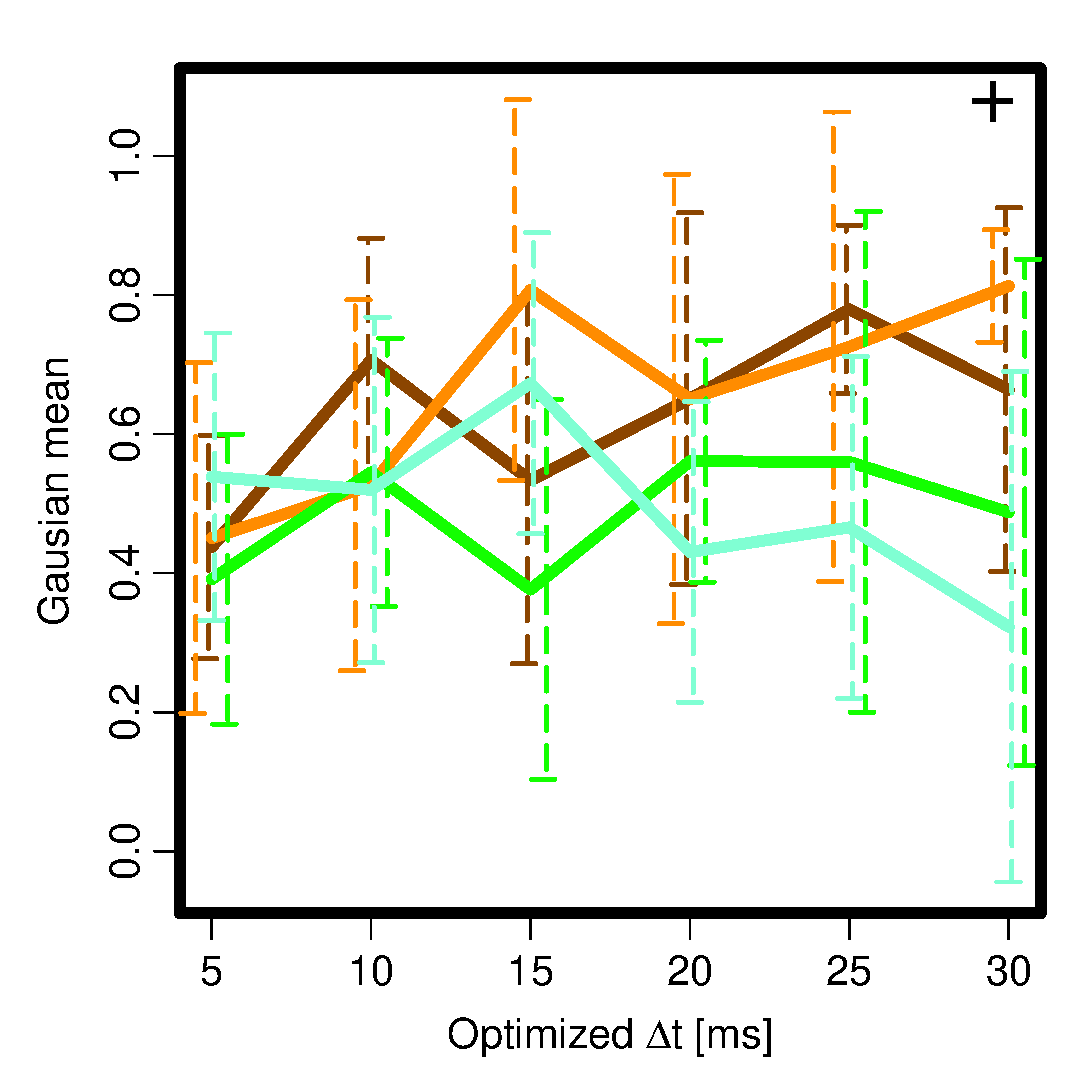
\includegraphics[width=0.8\columnwidth]{./Images_Result/k_Gaus_Upper_mean.eps}
         \caption{Upper Dendrite$B$N(BKa$B%3%s%@%/%?%s%9$N%T!<%/0LCV(B}
         \label{k_peak_upper}
       \end{subfigure}
       \begin{subfigure}{0.50\columnwidth}
         \centering
         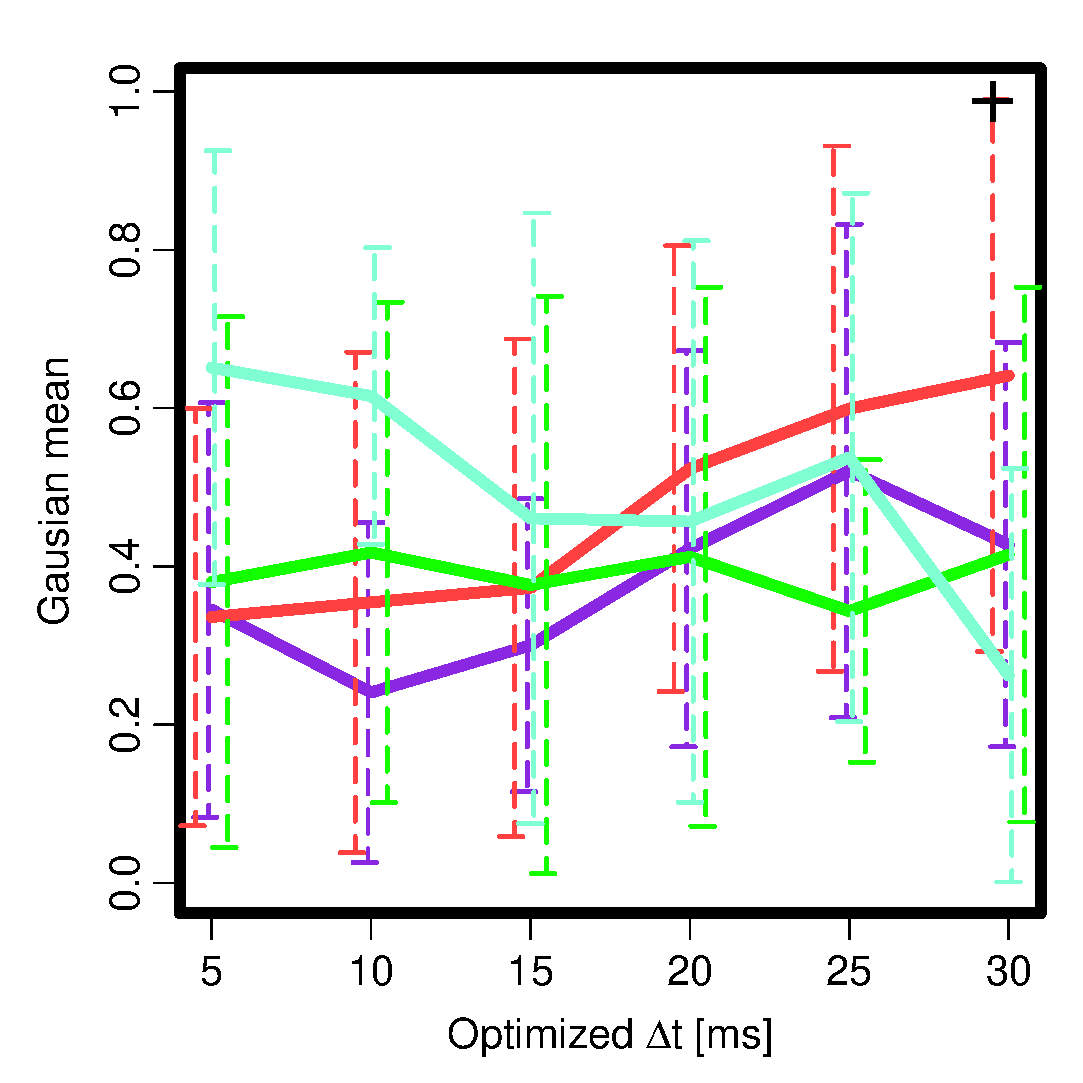
\includegraphics[width=0.8\columnwidth]{./Images_Result/ca_Gaus_Upper_mean.eps}
         \caption{Upper Dendrite$B$N(BCaT$B%3%s%@%/%?%s%9$N%T!<%/0LCV(B}
         \label{ca_peak_ca_upper}
       \end{subfigure}

       \begin{subfigure}{0.50\columnwidth}
         \centering
         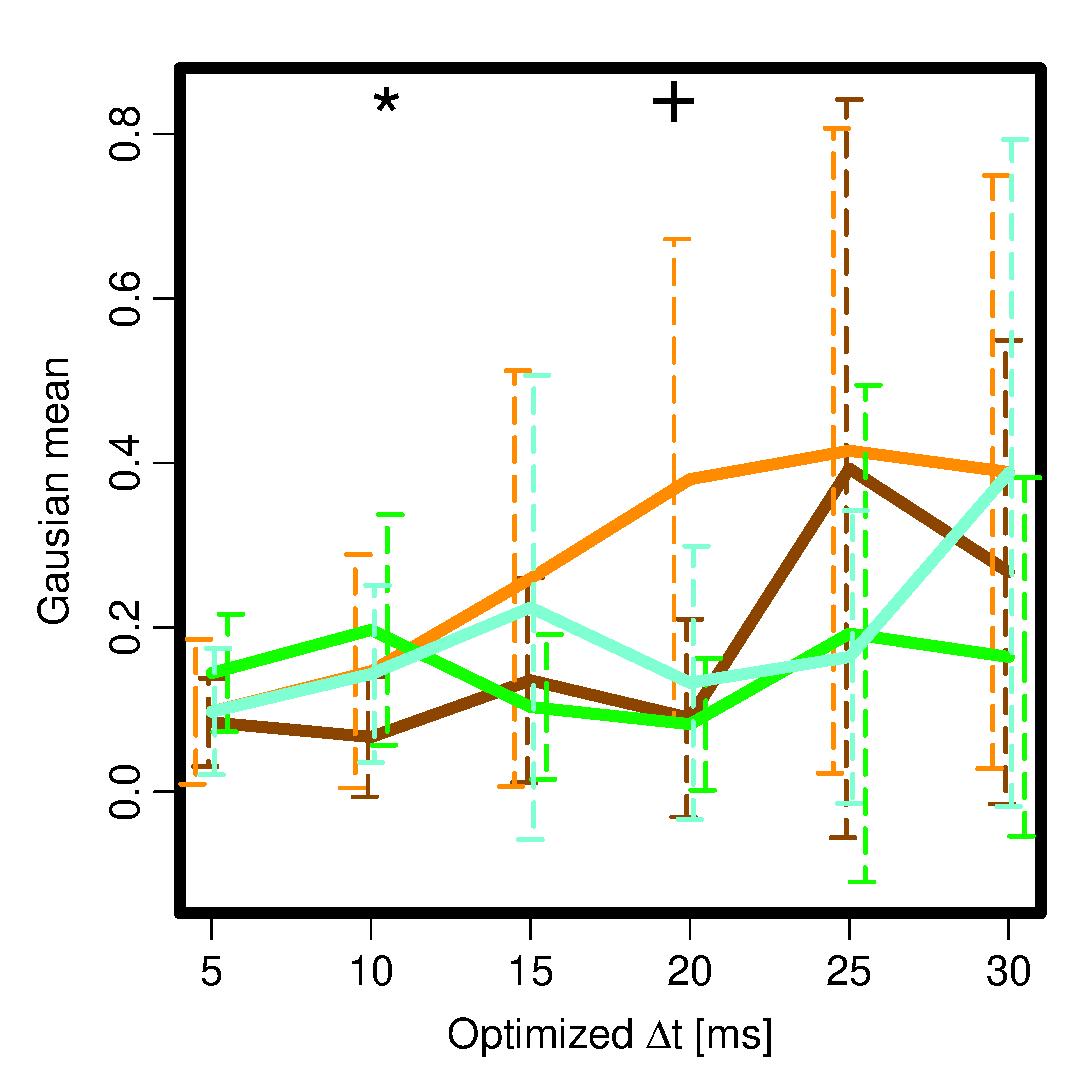
\includegraphics[width=0.8\columnwidth]{./Images_Result/k_Gaus_Lower_mean.eps}
         \caption{Lower Dendrite$B$N(BKa$B%3%s%@%/%?%s%9$N%T!<%/0LCV(B}
         \label{k_peak_lower}
       \end{subfigure}
       \begin{subfigure}{0.50\columnwidth}
         \centering
         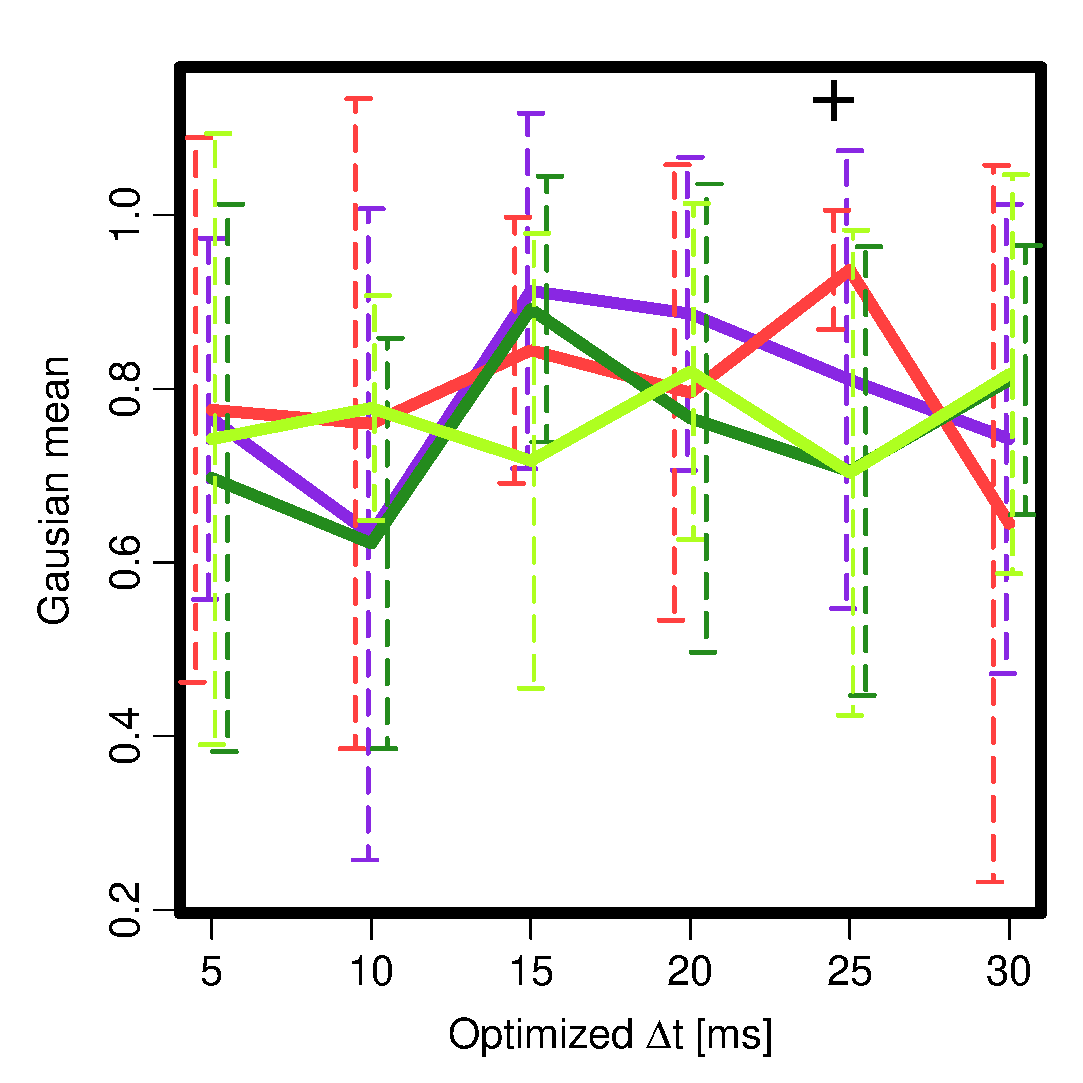
\includegraphics[width=0.8\columnwidth]{./Images_Result/ca_Gaus_Lower_mean.eps}
         \caption{Lower Dendrite$B$N(BCaT$B%3%s%@%/%?%s%9$N%T!<%/0LCV(B}
         \label{ca_peak_ca_lower}
       \end{subfigure}
       
       \begin{subfigure}{0.5\columnwidth}
         \centering
         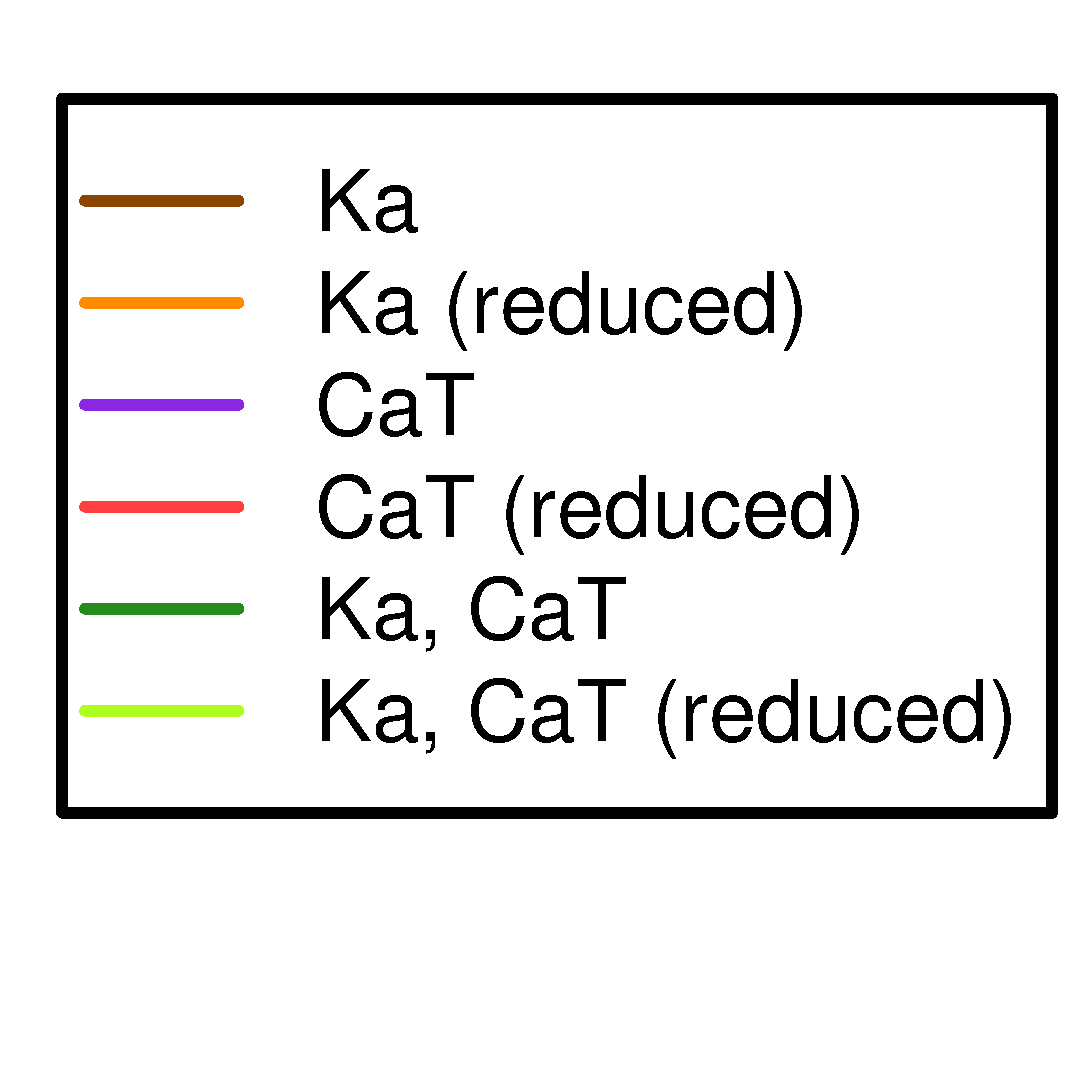
\includegraphics[width=0.5\columnwidth]{./Images_Result/Gaus_legend.eps}
       \end{subfigure}
       \begin{subfigure}{0.5\columnwidth}
         \centering
         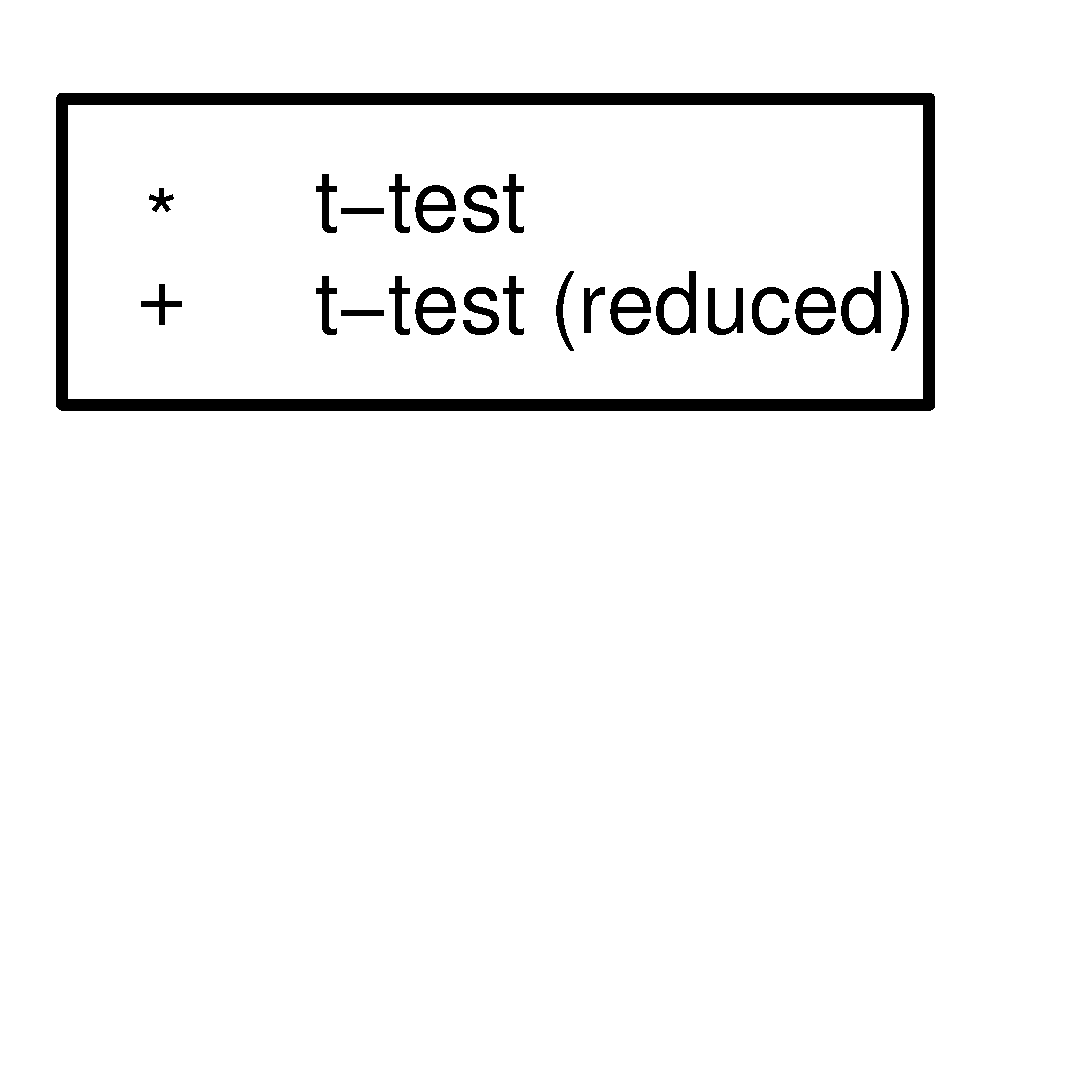
\includegraphics[width=0.5\columnwidth]{./Images_Result/Gaus_test_legend.eps}
       \end{subfigure}

       \vspace{-1cm}
       \caption{$B%,%&%9J,I[$rMQ$$$?(BKa$B%3%s%@%/%?%s%9$N%T!<%/0LCV(B}
       \label{Gaus_peaks}
     \end{figure}

     
